\documentclass[10pt,journal,compsoc,onecolumn, draftclsnofoot]{IEEEtran}

\usepackage{graphicx}
\usepackage{amssymb}
\usepackage{amsmath}
\usepackage{amsthm}
\usepackage{caption}
\usepackage{minted}

\usepackage{alltt}
\usepackage{float}
\usepackage{color}
\usepackage{url}

\usepackage{balance}
\usepackage[TABBOTCAP, tight]{subfigure}
\usepackage{enumitem}
\usepackage{pstricks, pst-node}

\usepackage{geometry}
\usepackage{pst-gantt}
\usepackage{tabu}

\usepackage{pdfpages}

\geometry{textheight=8.5in, textwidth=6in}
\graphicspath{ {./images/} }

%random comment

\newcommand{\cred}[1]{{\color{red}#1}}
\newcommand{\cblue}[1]{{\color{blue}#1}}


\usepackage{hyperref}
\usepackage{geometry}
\usepackage{array}
\usepackage{titling}

\def\name{Jake Jeffreys, McKenna Jones, Spike Madden, Sean Marty}
\title{
EmbarkVR: Outdoor Virtual Reality Experience \\
CS Senior Capstone \\
Final Report\\
\vspace{1mm}
}
\author{Jake Jeffreys, McKenna Jones, Spike Madden, Sean Marty}
\date{May 31, 2017}

%pull in the necessary preamble matter for pygments output

%% The following metadata will show up in the PDF properties
\hypersetup{
  colorlinks = true,
  linkcolor = black,
  urlcolor = black,
  pdfauthor = {\name},
  pdfkeywords = {``senior capstone''},
  pdftitle = {CS Capstone Report},
  pdfsubject = {CS Capstone Report},
  pdfpagemode = UseNone
}

\begin{document}
\begin{titlepage}
\maketitle
\vspace{1mm}
\begin{abstract}
This document summarizes the Outdoor Experiences in Virtual Reality project for the Computer Science Senior Capstone class at Oregon State University. In the document you will see original technical documents, weekly blog posts, project documentation and other general information regarding the project. We hope that this document will be equally valuable to high school students, future CS Capstone Students and the OSU CS department.

\end{abstract}
\vspace{1cm}

\end{titlepage}

\tableofcontents
% \let\tableofcontents\relax
\clearpage

\section{Project Overview}
This project was sponsored and proposed by Intel and Columbia Sportswear. The two stakeholders in the project are Mike Premi from Intel and Tim Devlin from Columbia Sportswear. Mike Premi served as the technical adviser, and Tim Devlin served as the conceptual adviser. The motivation behind the project is to both inspire people to get outdoors, and promote the Performance Fishing Gear line of fishing apparel by creating an immersive and interactive fishing experience. The members of the team, Jake Jeffreys, McKenna Jones, Sean Marty, and Spike Madden all contributed equally to documentation and development of the project. This project serves as a strong proof of concept of what a VR experience could look like in a retail space.

\section{Requirements}
\subsection{Original Requirements Document}
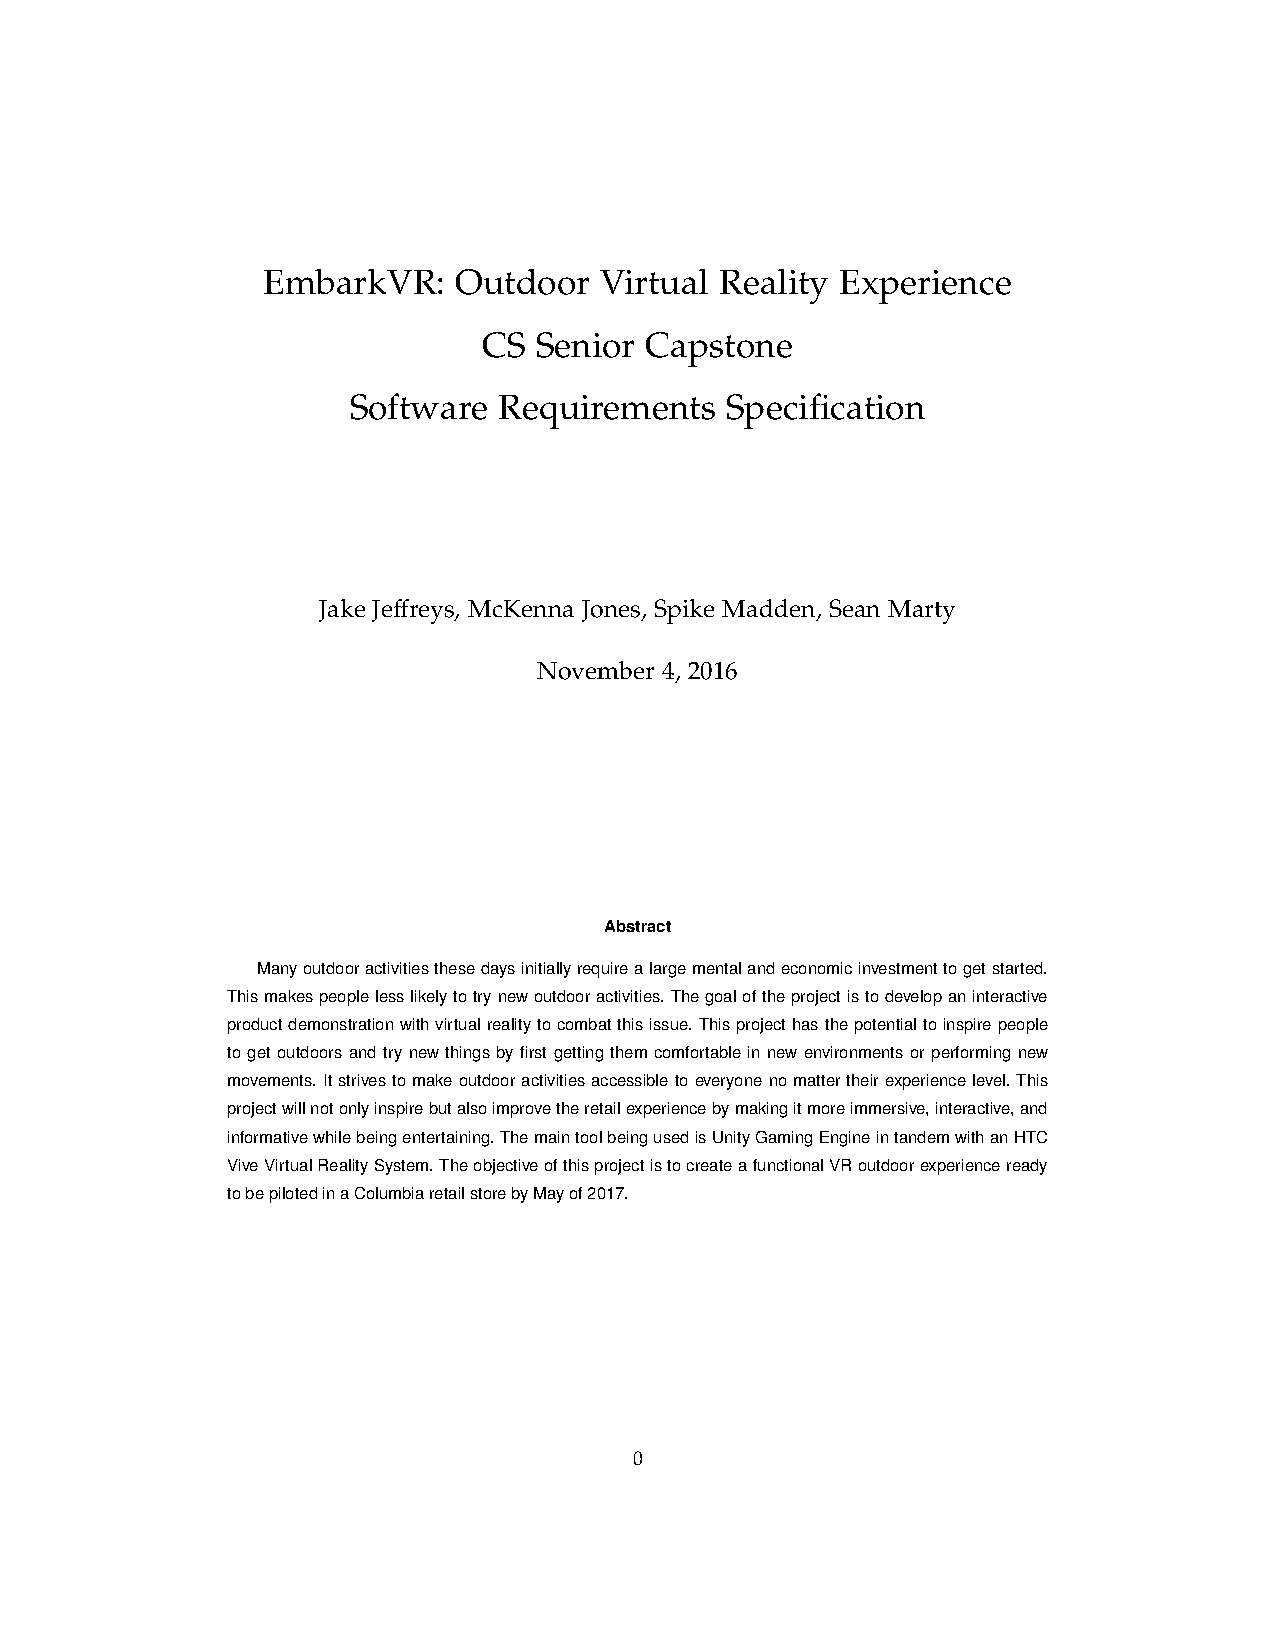
\includepdf[pages=-, frame, scale=0.9, pagecommand={}]{originalRequirementsDoc.pdf}

% TODO
\subsection{Requirements Document Changes}

\section{Design Document}
\subsection{Original Design Document}
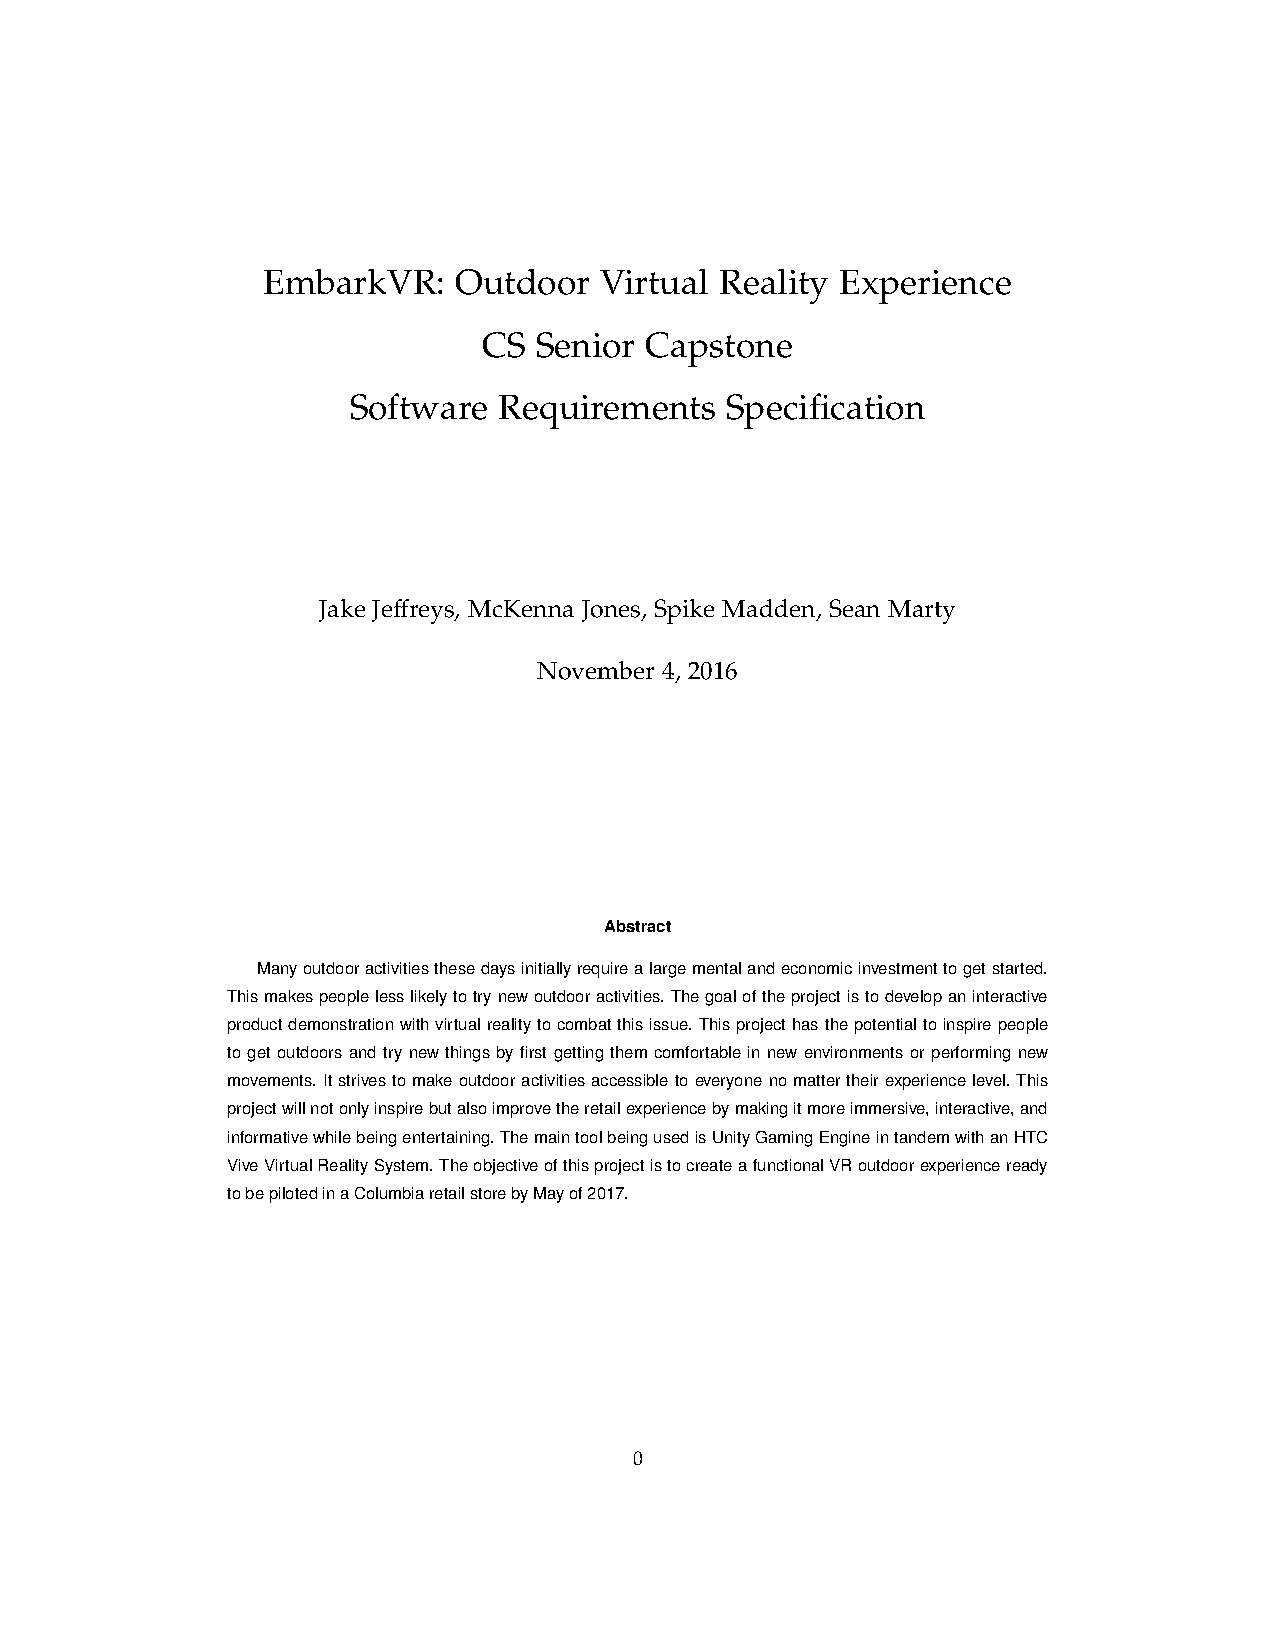
\includepdf[pages=-, frame, scale=0.9, pagecommand={}]{originalDesignDoc.pdf}

% TODO
\subsection{Design Document Changes}

\section{Tech Review}
\subsection{Original Tech Review}
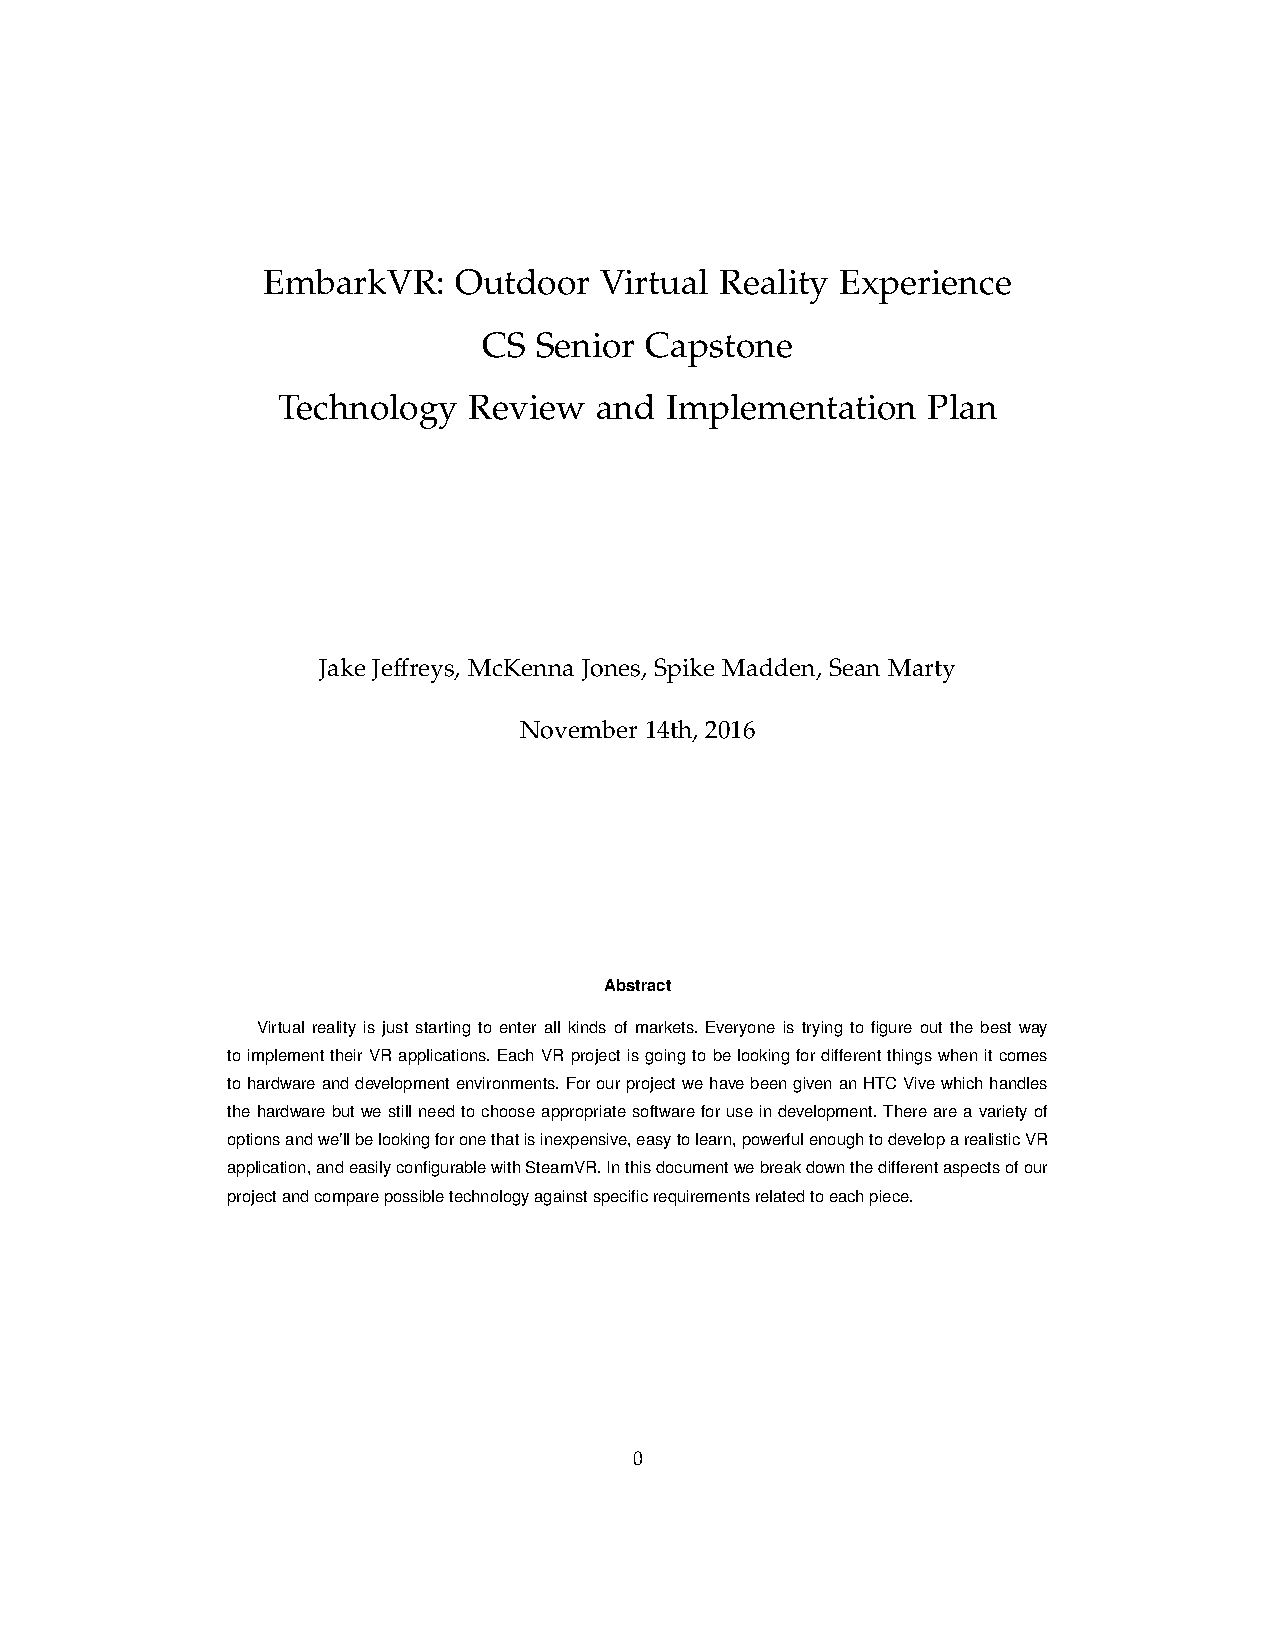
\includepdf[pages=-, frame, scale=0.9, pagecommand={}]{originalTechReview.pdf}

% TODO
\subsection{Tech Review Changes}

\section{Weekly Blog Posts}

\subsection{Fall Week 3}
\subsubsection{Jake}
\noindent \textbf{Week's Progress}

I spent the week putting together a Problem Statement which aimed to define the problem and make sure that everyone on the team and the sponsors are all on the same page. To help us write it we spoke with Mike and Tim over the phone and discussed their visions and the scope of the project.

\noindent \textbf{Problems Encountered}

Only problem we've faced so far is finding time that we are all free to meet and discuss the project with the sponsors. We have managed to find time but we'll need to make a big effort to be efficient we meet up.

\noindent \textbf{Plans for the Coming Week}

Next week I see the team starting to research the programs we'll be using and looking into getting our hands on a an HTC Vive.

\subsubsection{McKenna}
\noindent \textbf{Week's Progress}

This week we spent most of our time working on our problem statement. Overall this was a very smooth process. In order to complete this assignment we had a conference call with both of our sponsors: Mike Premi from Intel and Tim Delvin from Columbia. Our conversation with them served as the first meeting with our entire team. Before the meeting we only had a vague idea of what the project would entail. After the meeting the entire team was finally on the same page about the general details of the project. I would call this first meeting a huge success.

\noindent \textbf{Problems Encountered}

This week we did encounter any major road blocks. The main thing that held our team up was finding a time that was suitable for all of us to meet. With our of our busy schedules this was easier said than done.

\noindent \textbf{Plans for the Coming Week}

For this coming week we will continue planning our project. This will most likely be in the form of completing upcoming assignments for class, and talking with our sponsors more. The other thing we will most likely do is dive into VR and the Unity Engine. Currently another team which is working on a VR project with Intel has the HTC Vive and some other VR gear. Our team needs to coordinate a system for sharing this gear within the coming week.

\subsubsection{Sean}
\noindent \textbf{Week's Progress}

This week I worked with the team to formulate our Problem Statement. This included meeting up as a team, and having a conference call with our sponsors Mike Premi and Tim Delvin (referred to in the future as just Mike and Tim). We had to distill a bunch of information and big picture goals down into about a page of content explaining what we want to do.

\noindent \textbf{Problems Encountered}

No true problems faced this week.  A hard part of writing the Problem Statement was keeping our goals and deliverables vague enough to allow for the creativity and variability that is inherent in the project while also having something concrete to strive for.

\noindent \textbf{Plans for the Coming Week}

The biggest tasks I see coming this next week are to continue planning and following the process outlined by our capstone assignments, and learning about the Unity gaming engine.  Ramping up on Unity will help ensure I can hit the ground running once true development starts.

\subsubsection{Spike}
\noindent \textbf{Week's Progress}

Our team worked on the Problem Statement for our project which included an abstract, problem definition, proposed solution and performance metrics. To complete this week's assignment, the team had a conference call with Mike Premi from Intel and Tim Devlin from Columbia. We went over the vision and the goals of the project and discussed strategies on how to move forward.

\noindent \textbf{Problems Encountered}

We were unsure about the expected deliverables for this project but we were able to clear up our concerns during the conference call. Other than that, we didn't really have any large issues to deal with.

\noindent \textbf{Plans for the Coming Week}

We'll continue to brainstorm ideas for the project and work on the expected milestones for the class. The biggest technical short term goal for the team is to ramp on the Unity Engine so we're all familiar with its capabilities. We'll also have to contact the other Intel sponsored groups to work out times we can share the HTC Vive so we can do our own testing.

\subsection{Fall Week 4}
\subsubsection{Jake}
\noindent \textbf{Week's Progress}

I spent some time this week researching the software needed to create a Virtual Reality application. After finding the correct tools I looked into the hardware required to run these programs.

\noindent \textbf{Problems Encountered}

I currently work on a MacBook Pro from early 2011 which has the following stats:

- 2.3 GHz Intel Core i5
- Intel HD Graphics 3000 512 MB
- 8GB RAM

In the past I have had issues with Hd video editing but so far haven't had any major issues with Unity. I have experienced some lag so I will continue to keep an eye on it. Fortunately I will be investing in a new Computer with upgraded specs within the next month.

\noindent \textbf{Plans for the Coming Week}

Next week I will be working on the Requirements document and I will try to get in contact with Erik Watterson (a student on one of the other Intel VR Projects) to discuss usage of the HTC Vive gear.

\subsubsection{McKenna}
\noindent \textbf{Week's Progress}

The first thing I worked on this week was revising our problem statement. Luckily our problem statement was used as an example during class so we received some very valuable feedback from Kirsten. The main issue was our Problem Definition. We incorrectly thought that our problem was to create a VR experience. However, the root problem is to sell more Columbia Gear, which will be solved with our VR experience.

The other thing I did was work on getting the Unity Game Engine and Editor set up on my machine. For the most part this was a smooth process, and I have started to go though some basic tutorials to acquaint myself with the software.

\noindent \textbf{Problems Encountered}

The small problem I ran into this week was getting Unity on my laptop. I run Linux as my primary operating system, however, the Unity software is only officially supported by MacOS and Windows. I have both Windows and Linux installed on my machine so I was originally planning on having to dual boot to Windows every time I would want to do Unity development. Luckily, after a bit of searching I found a Unity Beta that had been released for Linux. It is the same version number as the official release so I should be fine developing on Linux. That being said, I am still unsure if my laptop is up to the task as it has no dedicated graphics card.

\noindent \textbf{Plans for the Coming Week}

For the coming week we plan to keep revising our problem statement. We will then also meet with our sponsors and discuss the changes we made.

\subsubsection{Sean}
\noindent \textbf{Week's Progress}

This week we worked to make edits to our Problem Statement.  Our document was used as an example in class, so we got some extra pointed feedback to go along with the feedback from Kevin.  Our biggest issue is a clear concise definition of what part of our problem statement actually needs to be our main "problem".  This mostly manifests as an ordering issue.  We have most all the info we need there, just not put together correctly.

\noindent \textbf{Problems Encountered}

No major problems faced this week other than being busy.  We need to edit our Problem Statement, but that was everyone in the class so I do not feel as though that is a major issue.

\noindent \textbf{Plans for the Coming Week}

Two big tasks for the coming week.  First, work to nail down requirements.  This keeps being stressed as super important for future success on the project so I don't want to put too little effort into it.  Second, I want to get familiarized with Unity game engine because that is the main area that we will be developing in once that starts up.

\subsubsection{Spike}
\noindent \textbf{Week's Progress}

We revised our Problem Statement slightly to accommodate for the changes that Kirsten suggested during class. I also downloaded the Unity Game Engine and messed around with some of the tools. It seems to run well which is really good.

\noindent \textbf{Problems Encountered}

I didn't really run into any problems this week since the only real task we had was to try to get Unity on our laptops. I didn't try any graphic intensive simulations so my GPU might become a problem, but so far it looks ok.

\noindent \textbf{Plans for the Coming Week}

We need to finish revising the Problem Statement so we can resubmit it for credit. We'll have to email our sponsors to outline the changes to make sure we're all on the same page. We should also continue to explore Unity.

\subsection{Fall Week 5}
\subsubsection{Jake}
\noindent \textbf{Week's Progress}

I met with Erik Watterson to learn about his project and to understand how to set up the HTC Vive. We also discussed the logistics of sharing the equipment. My team and I also created a rough draft of the requirements documentation for the project.

\noindent \textbf{Problems Encountered}

Erik and I came to the conclusion that it would be difficult for our two teams to share the same equipment for the entire project. The room the other team is using is also quite small so my team will probably need to find another location to set up our equipment.

\noindent \textbf{Plans for the Coming Week}

Next week I will work to create a final draft of the requirements document. I will also be looking for a location on campus my team can use to store our equipment once we get it.

\subsubsection{McKenna}
\noindent \textbf{Week's Progress}

This week we made progress in a few areas. First of all we finished up our Problem Statement based on suggestions from Kirsten, the TA's, and our clients. Secondly we developed a rough draft of our Requirements Document. Finally, we have made plans to get our own virtual reality gear from our clients. Before this there had been discussion of us sharing VR gear with another Capstone team who is also doing a VR project with Intel. While this would have been doable, it will be much easier if we have our own VR gear.

\noindent \textbf{Problems Encountered}

This week we did not run into any road blocks. The one thing that held us up a bit is that we still have many questions for our clients about the specifics of our project requirements. Once we get this information our Requirements Doc should come together nicely.

\noindent \textbf{Plans for the Coming Week}

For the coming week we plan to meet with our clients again and finish up our Requirements Doc.

\subsubsection{Sean}
\noindent \textbf{Week's Progress}

Met with our sponsors over Webex.  Talked about getting our own equipment instead of sharing with another Intel VR group, and about finalizing our Problem Statement.  We turned our problem statement in on time.  We worked some on the requirements document, still need a lot of work on it.

\noindent \textbf{Problems Encountered}

The requirements document is going to be very hard.  Just need to spend time thinking about it and working out each question.  The better we do with it, the easier the rest of the year will be.

\noindent \textbf{Plans for the Coming Week}

Big plans are to just make sure that we keep in good communication with our sponsors and keep up with the documents.  Also, need to continue ramping up on the Unity Game Engine.  There will be more info in next week's blog post, this week was relatively slow.

\subsubsection{Spike}
\noindent \textbf{Week's Progress}

We finished our revision of the Problem Statement after another meeting with our clients. We also worked on a Requirements Document with our clients and turned in a rough draft. We think we convinced our sponsor that our own VR system would be beneficial for the development of the project.

\noindent \textbf{Problems Encountered}

We didn't run into any huge problems this week. We still have some questions about the Requirements Document but we'll be able to get those answered as we figure out more of the in depth details of the project.

\noindent \textbf{Plans for the Coming Week}

We'll need to continue to work on the Requirements Document to clear up any of the ambiguous points. We should be getting access to our own VR system sometime soon, and it'd be great to set that up either on campus or one of our apartments.

\subsection{Fall Week 6}
\subsubsection{Jake}
\noindent \textbf{Week's Progress}

This week I was able to meet with Christian from one of the other Intel teams. I'm hoping we'll be able to do some collaboration through the year. He was able to bring down an HTC Vive, the stands, and a PC on Thursday for my team. That evening my Team and I were able to set up the HTC Vive and mess around with a few free applications. This week we were also able to complete the Software Requirements Specification for the project.

\noindent \textbf{Problems Encountered}

We had some issues completing the Software Requirements Specification. We are all new to VR and therefore lacked the knowledge needed to put this documentation together. Fortunately we were able to discuss this with our sponsors and find a few resources to help us.

\noindent \textbf{Plans for the Coming Week}

Next week we will being to ramp up with Unity development. Hopefully we'll be able to setup up an environment for us to work in as well as view our application from within the VR headset.

\subsubsection{McKenna}
\noindent \textbf{Week's Progress}

This was a busy week for our team. First we got our problem statement back which we did not do as well as we thought we did on. Lucklily we can still revise it and resubmit it. Secondly, we recieved our VR gear. This was huge for us. It was the first time that all of use got to try VR. Intel was very generous with the gear that they lent us. Finally we spent most of the week finishing up our requirements document.

\noindent \textbf{Problems Encountered}

We encountered one road block this week related to our requirements document. We struggled to nail down quantitative performance requirements. Us and the clients agreed that the VR experience should be as realistic as possible. The problem is that this is a hard thing to measure. The one quantitative performance requirement that we came up with is to make sure that our experience runs at at least 60 frames per second.

\noindent \textbf{Plans for the Coming Week}

For the coming week we plan on exploring VR much more and getting ready for the tech review.

\subsubsection{Sean}
\noindent \textbf{Week's Progress}

We updated our rough draft and turned in a final copy.  This was more of a struggle than we had thought it would be, mostly in the area of finding quantitative measures for how "real" our experience is. In the end we settled on our major "real-ness" measure being frames per second.  Also, we were delivered our virtual reality hardware on Thursday.  We signed up for Vive software and set up the physical headset.  The first demo we ran through was AWESOME!

\noindent \textbf{Problems Encountered}

The requirements document proved to be very difficult for our group, although working through them was a great exercise. We have plenty of subjective requirements but not as many objective ones. I don't know if it counts as a problem for this week, but before we got our HTC Vive, it was a little hard to put what we were writing and thinking about in context.

\noindent \textbf{Plans for the Coming Week}

I am so excited to get better at Unity and be able to build something and then bring it to life in our Vive!  Getting our VR setup working will open up so much more for our ramping on Unity.  I also want to get more ahead on the documentation so that we aren't cutting it so close on the deadline this next time.

\subsubsection{Spike}
\noindent \textbf{Week's Progress}

We completed our Requirements Document after revising the draft we submitted for feedback. We met with our TA and clients to discuss specifics within the document and I think we've done a good job of outlining our requirements. A huge step in progress came on Thursday when we actually received VR gear including the headset and a VR ready laptop. Setup went smoothly and the components seem to be working well.

\noindent \textbf{Problems Encountered}

We had some issues when it came to the performance metrics in the Requirements Document. We couldn't figure out how to quantify how realistic or how immerse the VR environment we were creating would be . After meeting with our TA, we did some extra research and tried to keep our performance metrics as quantifiable as possible.

\noindent \textbf{Plans for the Coming Week}

We have the VR station set up so we'll continue to ramp on Unity and start to develop scenes that we can actually test on the system. A basic environment in Unity that can be tested with the Vive could be a possibility.

\subsection{Fall Week 7}
\subsubsection{Jake}
\noindent \textbf{Week's Progress}

This week we were able to experiment with Tilt Brush by Google. This application does an amazing job of handling the user experience. Tilt Brush offers an incredibly user friendly way to interact with a 3d paint brush. It is intuitive and every single person on my team was able to understand exactly what to do within 10 seconds. Moving forward we will strive to incorporate similar ideas into our project. This week I also wrote 3 pieces for the Technology review.

\noindent \textbf{Problems Encountered}

The main problem I had this week was finding time to setup an development environment. I think the Technology review could be helpful for some groups but for us, since we've already spent time choosing our technology, is a complete waste of time. It has taken away from us being able to move forward on the project.

\noindent \textbf{Plans for the Coming Week}

Next week I hope to complete the Technology Review and have a completed Gantt chart. This gantt chart will be incredibly valuable in helping us plan out our project to get an idea of we is possible in the time frame.

\subsubsection{McKenna}
\noindent \textbf{Week's Progress}

This week we continued to experiment with VR. We've been playing some of the most popular titles from Steam Store. Playing these polished games has given us a lot of ideas for features that we would like to implement in our game. For example, we have seen many different ways to display menus, some good and bad. Similarly, we have seen a couple different ways that developers deal with teleporting in game. Most of our other time this week has been spent working on the Tech Review

\noindent \textbf{Problems Encountered}

We didn't experience any major problems this week. The one thing we struggled with a bit was how to structure our Tech Review. For most of our project we will be making use of the Unity Game Engine. Therefore, for our Tech Review we simply decided to compare how we would implement features in different gaming engines.

\noindent \textbf{Plans for the Coming Week}

For the coming week we hope to implement a "Hello World" type of program in Unity. This will be our first try at developing in Unity.

\subsubsection{Sean}
\noindent \textbf{Week's Progress}

This week was a little bit rough.  Mostly worked to figure out what the heck we are going to do for our tech review.  We divided up tasks into four sections, one for each of us to write about.  This also included working through some questions about which sections would require the most work.  Also kept ramping up on Unity when time allowed.

\noindent \textbf{Problems Encountered}

I faced two main problems.  First, I think our group is a little bit behind.  It feels like we are reaching just to complete each document, and that is taking up most of our available time that we should be using more of to ramp up on Unity and get a prototype out.  Second, it feels like those of us also in other classes with McGrath are getting a huge load of work dumped on us kind of out of nowhere.  This is making it stressful to get everything done on time.

\noindent \textbf{Plans for the Coming Week}

Just to work as fast as possible to get the tech review done and start busting out more learning on Unity.  Hopefully I can get a Hello World sort of environment with some basics going by the time I leave for Thanksgiving break.  We will see.

\subsubsection{Spike}
\noindent \textbf{Week's Progress}

We spent a lot of this week getting more familiar with the Vive and trying out new games. We got assigned the Technology Review document so the team brainstormed some tasks. The big sections we came up with are: the environment, wand/rod usage, Columbia products and the UI and user guide.

\noindent \textbf{Problems Encountered}

The Technology Review document is a little troubling because our team has settled on using Unity with the Vive as that's what our clients suggested. We'll be looking at different development environments as well as different strategies within Unity but this assignment seems a little pointless.


\noindent \textbf{Plans for the Coming Week}

We'll be finishing up the Technology Review document this weekend and attempt to build a basic working prototype in Unity. We're looking to build a simple environment with maybe some objects the user can interact with.

\subsection{Fall Week 8}
\subsubsection{Jake}
\noindent \textbf{Week's Progress}

This week we completed the Technology Review. We were also able to set up a development environment to begin building our VR application. Fortunately there is a SteamVR plug-in in the Unity asset store which makes testing our application within the VR experience quick and easy.

\noindent \textbf{Problems Encountered}

No major problems this week but we will need to figure out how to quickly, effectively, and cheaply create a realistic outdoor environment. It looks like a lot of the more realistic assets cost money so we will need to do some research into other ways.

\noindent \textbf{Plans for the Coming Week}

Next week I hope to figure out what our environment should look like and how it should all be laid out. It would also be great if we were able to find free tools that can autogenerate landscapes and environments which we could then use as a template to build on.

\subsubsection{McKenna}
\noindent \textbf{Week's Progress}

This week we made progress in a few areas. First we finished out Tech Review on Monday. For us, this document ended up being very repetitive because most of our project will be completed in Unity and we were pretty much set on using Unity before starting the document. However, it was still a good exercise to explore how other gaming engines impliment certain features. This week we also completed a "Hello World" type program in Unity. We were able to create a simple environment using basic assets from the Unity Asset Store and view that in the HTC Vive headset. This was a big step for us.

\noindent \textbf{Problems Encountered}

We did not encounter any problems this week.

\noindent \textbf{Plans for the Coming Week}

For the coming week we plan to start our Design Document and continue experimenting with Unity.

\subsubsection{Sean}
\noindent \textbf{Week's Progress}

Finished and turned in tech review.  Got a real "hello world" environment ported into SteamVR so we can explore it in our Vive headset.  Started exploring more of the documentation and tutorials for building experiences in Unity.

\noindent \textbf{Problems Encountered}

The tech review was hard.  We did it, but it was hard.  For me, it was kind of a weird exercise because we were doing 500-1000 words for each section, and to feel like I did a thorough job on a topic like I tackled, I would need to do many times that and spend weeks.  But it was still good to start working through documentation and delving deep into the nitty gritty.

\noindent \textbf{Plans for the Coming Week}

Build up a working prototype of the environment just so we can teleport around and explore while in virtual reality. Also, settle on whether we want to have our project documented for OSU.  We need to set up a meeting for the week after Thanksgiving with our sponsors just to check in with them and ask any questions.  Nothing specific to ask, more just to keep them updated and keep up good communication.

\subsubsection{Spike}
\noindent \textbf{Week's Progress}

We got a couple tasks done this week. We finished up our tech review document on Monday. A lot of it was repetitive where we talked about different gaming engines (Unity, Unreal Engine 4, Lumberyard) for the three different technologies. Our clients are asking us to use Unity so the document was a little tedious. We also were able to load a basic environment, made in Unity, onto the Vive.

\noindent \textbf{Problems Encountered}

There were no problems we ran into this week.

\noindent \textbf{Plans for the Coming Week}

We'll be working on the Design Document this week and improving the environment we've built.

\subsection{Fall Week 9}
\subsubsection{Jake}
\noindent \textbf{Week's Progress}

I put together a statement about my fears and excitements for our project. I also talked with Mike Premi about our Technology Review and about getting NDA agreements for our team so we can collaborate more with Erik's team.

\noindent \textbf{Problems Encountered}

The only problem I encountered was Erik's team is a little hesitant to collaborate with us since we haven't signed NDA agreements.

\noindent \textbf{Plans for the Coming Week}

Next week I plan to work on the Design Document and begin thinking about the final Progress Report.

\subsubsection{McKenna}
\noindent \textbf{Week's Progress}

This week we continued to develop our prototype environment in Unity. We are learning new aspects of the engine rapidly from online tutorials. We also continued to work on the Design Doc, but we still have a lot of work to do before the due date next Friday.

\noindent \textbf{Problems Encountered}

We did not encounter any problems this week.

\noindent \textbf{Plans for the Coming Week}

For the coming week we plan to spend most of our time finishing up the Design Document. One of our project sponsors also suggested that we look into the Singray Gaming Engine, so we will experiment with that a bit.

\subsubsection{Sean}
\noindent \textbf{Week's Progress}

This week was relatively quiet as a group.  Most of my time was spent just doing some research and work on a basic prototype. I started looking into the Design Doc but I have not had a ton of time to work on it.

\noindent \textbf{Problems Encountered}

First off, this wiki post was supposed to be done this last Friday, but being the day after Thanksgiving and this weekend being kind of hectic I forgot.  Second, I was away from the HTC Vive headset and all of our VR equipment so this week was a little bit hard to get much progress done on actual prototype development.  Lastly, I am scared that we haven't done enough implementation to truly write a good Design Document.

\noindent \textbf{Plans for the Coming Week}

I am going to try and push some implementation this Monday and Tuesday, while also buckling down on Design Doc work.  Hopefully have the Design Doc done and ready for review by Mike and Tim Wednesday night by the latest. Also, I want to spend time each day this week mapping out topics, content, etc for our poster and term presentation.

\subsubsection{Spike}
\noindent \textbf{Week's Progress}

We worked on our prototype of the natural environment in Unity. I looked up some VR fishing games on YouTube to check out the interaction of the wands and rod. We did a little work on the Design Document but we'll have to finish that up this week.

\noindent \textbf{Problems Encountered}

We didn't encounter any problems this week.

\noindent \textbf{Plans for the Coming Week}

We'll be working on the Design Document this week. We'll probably also improve on the prototype of the basic environment that Sean created in Unity.

\subsection{Fall Week 10}
\subsubsection{Jake}
\noindent \textbf{Week's Progress}

This week I created a design document to plan out the entire development process. My team also reached out to the other VR team to discuss future collaboration opportunities.

\noindent \textbf{Problems Encountered}

The only problem we encountered this week was trying to figure the requirements for our design document. The instructions were incredibly unclear and it seemed like everyone was telling us something different.

\noindent \textbf{Plans for the Coming Week}

Next week I plan to start working on the prototype. This will continue into the following week.

\subsubsection{McKenna}
\noindent \textbf{Week's Progress}

This week all of our time was devoted to developing our design document. We had hoped to spend some time working on our prototype in Unity, but with the chaos of dead week, this didn't happen.

\noindent \textbf{Problems Encountered}

We struggled quite a bit with the format of our design document. First of all, the IEEE format document was not clear at all. This was made worse by the fact that some of the professors recommended a completely different format. In the end we ended up with something that made sense to read, but may not fit the IEEE format correctly.

\noindent \textbf{Plans for the Coming Week}

For the coming week we plan to spend time working on our progress report. After that is done we are going to spend a few days of our winter break flushing out a prototype because we will all have free time for once.

\subsubsection{Sean}
\noindent \textbf{Week's Progress}

This week we wrote our entire design document, which was super helpful for getting the details of our project into focus. Also, we finally got a real good meeting with Erik Watterson and his team to collaborate on our similar VR projects.

\noindent \textbf{Problems Encountered}

Not too many problems actually! We need to sign the NDA for Erik's project so that we can more easily collaborate, but other than that no issues!

\noindent \textbf{Plans for the Coming Week}

We have the final projects due, and then just work a bunch on the actual implementation!

\subsubsection{Spike}
\noindent \textbf{Week's Progress}

We started and finished our design document. We haven't gotten the signatures yet but our finished document was turned in on time. We didn't have any time to work on the prototype.

\noindent \textbf{Problems Encountered}

We ran into a lot of troubles with formatting the design document. The IEEE format wasn't clear, and the professors said to disregard a lot of the information provided on the assignment sheet. We were able to complete it, and hopefully it's in a passable format.

\noindent \textbf{Plans for the Coming Week}

We need to finish up the progress report. This includes the written presentation and a recorded presentation. After that, we should have some time to work on our prototype in Unity.

\subsection{Winter Week 1}
\subsubsection{Jake}
\noindent \textbf{Week's Progress}

Over the break we were able to create our first prototype. It involved a terrain, trees, water animation, first person VR view, and minor touch mechanics with the VR controllers. The first week of this term we fixed an issue with our trees, we expanded our terrain to improve realism, and started adding direction to the water. As a team we also decided on weekly meeting times throughout each week to work on the project.

\noindent \textbf{Problems Encountered}

One problem we ran into was adding direction to the water that would match the curves of the river. We will continued to research solutions and try combining multiple water objects.

\noindent \textbf{Plans for the Coming Week}

Next week I plant to meet with the TA for the first time since last term. We will also reach out to our clients to set up more regular conference calls. We will continue to develop the terrain and improve our river feature.

\subsubsection{McKenna}
\noindent \textbf{Week's Progress}

This week we continued work on the prototype that we had started over winter break. We made progress by enlarging the terrain and making it generally more realistic. We also sat down and figured out good meeting times for our group throughout the term.

\noindent \textbf{Problems Encountered}

We are still a little shaky on how we will be actually incorporating the Columbia Sportswear gear into our experience. We will be meeting with our project advisors soon to figure this out.

\noindent \textbf{Plans for the Coming Week}

This coming we will continue to work on our prototype. We are also planning on meeting with our project advisors and possibly the other VR team at OSU to see where they are in their project.

\subsubsection{Sean}
\noindent \textbf{Week's Progress}

I did not get a lot done this week, but we met as a team and set up when we wanted to meet and how often.  We also talked a little bit about our general strategy for attacking this term.

\noindent \textbf{Problems Encountered}

Not many problems encountered, mostly just that we only have 10 weeks and we need to get rolling on this.  We also need to get our NDA with Intel sorted out if we are going to work with Erik Waterson's team to combine knowledge.

\noindent \textbf{Plans for the Coming Week}

This week I plan to watch a ton of tutorials and just get more versed in basic development for VR, as well as how to create an awesome static environment. Just basically attacking every problem I can this week.

\subsubsection{Spike}
\noindent \textbf{Week's Progress}

We have a working prototype of the static environment in Unity and we spent a little time this week working on that. We met up as a group to talk about meetings and also created a rough list of tasks we want to accomplish soon.

\noindent \textbf{Problems Encountered}

We had some trouble with water textures and the trees within the virtual environment. We got those sorted out but we'll have to continue working on that.

\noindent \textbf{Plans for the Coming Week}

We'll continue to work on our environment in Unity. We also have plans of setting up a conference call with our sponsors to catch up on our progress and figure out what's next.

\subsection{Winter Week 2}
\subsubsection{Jake}
\noindent \textbf{Week's Progress}

This week we first reached out to our clients to begin setting up weekly or biweekly meetings. We also all met as a team multiple times to create a plan moving forward and to set out initial design goals. These mainly involved creating a new river and adding new rocks and plants.

\noindent \textbf{Problems Encountered}

The main problem we ran into was that we are unsure whether or not to commit a lot of time to building our own assets or requesting a budget to purchase prebuilt assets so that we can focus on more import development.

\noindent \textbf{Plans for the Coming Week}

Next week I hope to talk with Mike and Tim to discuss assets and a possible budget. I hope we are also able to develop a routine moving forward where each team member has their own section of the project to be working on.

\subsubsection{McKenna}
\noindent \textbf{Week's Progress}

This week we made progress in a couple areas. First of all we began working on making the water of river more realistic. We found one free Unity package that seems promising. We also began making the foliage more realistic. This will primarily be in the form of bushes and grass around the river. Finally, we approached our clients about setting up biweekly meetings.

\noindent \textbf{Problems Encountered}

We have realized that without a budget to buy assets, we will spend most of our time manually building assets. It would be much more beneficial to spend our time working on other interesting aspects of the project.

\noindent \textbf{Plans for the Coming Week}

This coming week we need to meet with our clients to discuss a possible budget to buy assets. We would also like to meet with them to discuss the specifics of incooperating Columbia gear into the project.

\subsubsection{Sean}
\noindent \textbf{Week's Progress}

We met a couple times as a team to just start attacking our development head on. Built out and refined the landscape a bit, and learned a lot more about availability and usability of external assets.

\noindent \textbf{Problems Encountered}

We are going to need either assets from Columbia/Intel, or a budget to buy nicer asset packages.  We need to do this to bring our environment to life, and to include Columbia products in our experience.

\noindent \textbf{Plans for the Coming Week}

Build out the environment a bit with what we have, but don't go too far until we nail down final assets etc. Just mainly put in as many hours as possible learning about the whole development process and each facet.

\subsubsection{Spike}
\noindent \textbf{Week's Progress}

The team met up a couple times to work on the environment. We've been experimenting with different water shaders and tree/rock combinations. We emailed our sponsors to update them on our progress.

\noindent \textbf{Problems Encountered}

We're having trouble incorporating Columbia products within the VR environment. We're either going to need to get assets from our sponsors or figure something out with them in the coming weeks. It'd also be nice to have a small budget to purchase some high quality assets for the fly fishing environment.

\noindent \textbf{Plans for the Coming Week}

We'll continue to work on our Unity project but we really need to have a conference call with our sponsors to sort out the problems we're running into.

\subsection{Winter Week 3}
\subsubsection{Jake}
\noindent \textbf{Week's Progress}

This week we worked on building up our environment with foliage and rock features. We also started creating a vision for how we want our final application to look.

\noindent \textbf{Problems Encountered}

One problem we encountered was the rendering distance while in the development view. We were having a hard time adding grass to our terrain because we couldn't see where we had already placed it.

\noindent \textbf{Plans for the Coming Week}

Still haven't heard from Mike or Tim so next week I hope to talk with them to discuss assets and a possible budget. Just like last week I hope we are also able to develop a routine moving forward where each team member has their own section of the project to be working on.

\subsubsection{McKenna}
\noindent \textbf{Week's Progress}

This week we continued to improve the realism of our terrain. This was primarily in the form of grass and rocks around the river. We also made some initial progress in implementing user interaction with objects in the environment. To do this we used a Unity package called NewtonVR which is a physics based VR interaction system that supports the Vive very well.

\noindent \textbf{Problems Encountered}

We have yet to hear from our project sponsors after emailing them over a week ago. This is a litte concerning because there are some things that we really need to discuss with them in order to begin making more progress on the project.

\noindent \textbf{Plans for the Coming Week}

This coming week we hope to meet with Mike and Tim. We need to discuss a budget to buy assets, and the details regarding how we will include Columbia gear into the experience. We will also continue to work on the user interaction and realism parts of the project.

\subsubsection{Spike}
\noindent \textbf{Week's Progress}

We continued to work on the environment and a little work on interaction with objects with NewtonVR. Jake had a cool idea of creating a "campsite" location in the VR environment to showcase the Columbia gear. We'll start implementing that.

\noindent \textbf{Problems Encountered}

The environment is looking decent but paid assets, especially for the water, could be really helpful. We also don't have access to any Columbia assets yet so it's hard to incorporate that part of the project into our design.

\noindent \textbf{Plans for the Coming Week}

We emailed our sponsors but we haven't gotten a response yet. It'd be really good to have a conference call to share out progress and to have Tim send us some Columbia assets that we could use. It'd also be nice to have a budget so we could purchase some paid assets from Unity's Asset Store.

\subsection{Winter Week 4}
\subsubsection{Jake}
\noindent \textbf{Week's Progress}

This week we thought about our end goal. We then proceeded to divide up the project into four major sections and assign these to group members. I am responsible for the campsite which is the location where the user will start out. This will be where the user gets comfortable and can inspect Columbia gear. So far I've created a flat location and added some free example assets. I also carved out a road that leads to the campsite.

\noindent \textbf{Problems Encountered}

One problem I encountered was that there are very few quality, free assets available. I placed sample assets throughout the campsite as placeholders.

\noindent \textbf{Plans for the Coming Week}

Plan to talk with Mike and Tim on Monday and discuss a possible budget. As a team we also plan on consolidating our work and making more plans for the future.

\subsubsection{McKenna}
\noindent \textbf{Week's Progress}

This week was primarily a planning week for our team. We all got together and made sure that it was clear who is responsible for each part of the project. I think this was a big step for us. I will primarily be working on the fishing rod. We also made a decision to make the main part of our experience be a campsite where the user can view and interact with Columbia gear. This gives us much more freedom compared to having the experience be centered around fly fishing.

\noindent \textbf{Problems Encountered}

We heard back from one of our clients, but have yet to hear back from the other client. Therefore, we were once again unable to meet to discuss the project this week. This has been a significant roadblock for us. It has been a large amount of time since we met with our clients.

\noindent \textbf{Plans for the Coming Week}

This coming week we will finally meet with Mike and Tim to discuss the project. We will also all continue to work on our individual aspects of the project.

\subsubsection{Sean}
\noindent \textbf{Week's Progress}

Met with Vee on Monday (finally, I had missed the previous one so this was my first). Also went to class for the first time in a while. Good to get back and locked in. My team corresponded with our sponsors to set up a regular winter term weekly conference call.

\noindent \textbf{Problems Encountered}

Still facing an issue of not having the funds for good asset packages.  Hopefully a conference call with our sponsors this coming week will clear things up in that manner.

\noindent \textbf{Plans for the Coming Week}

This weekend I plan to get my personal laptop all up to speed so I can begin working on my individual section of the project. I want to make a bunch of progress this week while I have a relatively quiet week.

\subsubsection{Spike}
\noindent \textbf{Week's Progress}

This was a slower week but we got some good planning done. We created a rough schedule of certain tasks that need to be completed to be able to produce a working beta by the end of this term. I'm in charge of Columbia products and the product display interface so I did some research on menus and other UI elements in Unity.

\noindent \textbf{Problems Encountered}

We didn't run into any problems this week.

\noindent \textbf{Plans for the Coming Week}

We have a conference call with our Columbia sponsor, Tim, next Monday. We'll be able to ask a lot of the questions we've been mentioning in our previous blog posts. The biggest things are: a budget for Unity assets, Columbia product assets and scheduling a time to visit.

\subsection{Winter Week 5}
\subsubsection{Jake}
\noindent \textbf{Week's Progress}

This week we had a conversation with Tim about project goals and direction. We will be moving away from displaying gear and more towards a physical experience (fly fishing, cutting wood, skipping a rock). I also spent time working on building up the campsite as well as helping to scale the landscape.

\noindent \textbf{Problems Encountered}

One problem we encountered was that the direction we were going was slightly off since Columbia already has VR applications that display gear. Instead we will be creating interactive experiences.

\noindent \textbf{Plans for the Coming Week}

I plan to finish the campsite boundaries and begin working on object interaction. I hope we can talk with Mike and Tim again to bounce some ideas off of them.

\subsubsection{McKenna}
\noindent \textbf{Week's Progress}

This week we were able to meet with on of our sponsors, Tim, from Columbia. This meeting was very productive. In this next couple days Tim will be providing us with assets of Columbia apparel that we will be able to use in our project. We also discussed the possibility of a small budget for our team, which will allow us to buy some higher quality assets, that will improve the realism of our project. Finally, we decided that user movement, in the form of fishing and possibly other activities should be the focus of our project.

I also made some small strides on the fishing aspect of the project. I am able to "cast" a line. It's a simple rigid line for now, but it's a start.

\noindent \textbf{Problems Encountered}

The meeting we had this week did steer our project in a slightly different direction than we were initially working towards. However, it is better to change direction now rather than in a few weeks.

\noindent \textbf{Plans for the Coming Week}

This coming week I plan to continue working on the fishing aspect of the project.

\subsubsection{Sean}
\noindent \textbf{Week's Progress}

We met briefly with Vee on Monday, not a lot there. Much more importantly, had a conference call with Tim (Columbia client) and got a lot more clarity on how to go forward. This was good because it had been a little while since we had spoken to our client "in person" (not email).

\noindent \textbf{Problems Encountered}

No major issues. A little bit of a change of direction based on the talk with Tim, but that is a good thing not really a problem. We still have the issue of not enough assets, but we worked out a tentative fix with Tim.

\noindent \textbf{Plans for the Coming Week}

This week the main focus is continued development and also work on a set of assignments for the class portion of capstone. For development, I want to finish up the environment using the assets we currently have.  Get it to a state where we can take some screen shots or even video as an update for clients and Github.

\subsubsection{Spike}
\noindent \textbf{Week's Progress}

We had a call with our Columbia sponsor, Tim Devlin, to catch up with our progress. We discussed his vision for the project, the availability of Columbia assets and a budget for other assets to improve the aesthetic of our environment.

\noindent \textbf{Problems Encountered}

After talking with Tim, it looks like we have to change the direction of our project. We originally thought the main goal of this VR project was to promote Columbia gear, but it seems like the interaction/fishing portion is what's really important. We'll have to make some minor adjustments to account for this.

\noindent \textbf{Plans for the Coming Week}

We'll continue to work on the fishing experience as there's a bigger focus on that now. We should be getting the Columbia assets sometime in the upcoming week so we can work to add those to the scene as well.

\subsection{Winter Week 6}
\subsubsection{Jake}
\noindent \textbf{Week's Progress}

This week I continued developing the campsite. In general, development was put on hold this week to work on our midterm progress report. We created a progress report and a video to accompany it showing what we have done so far.

\noindent \textbf{Problems Encountered}

No major roadblocks this week as we spent most of our time on documentation rather than development.

\noindent \textbf{Plans for the Coming Week}

This upcoming week I hope to finish the boundaries of the campsite, experiment with sky textures, and get approval for some low cost assets.

\subsubsection{McKenna}
\noindent \textbf{Week's Progress}

This week we spent the majority of our time finishing up both the written and video portions of our progress report. This was a bit frustrating because it took away a lot of time from development, however it was beneficial to reevaluate where we are in the project. I also made some small strides with the fishing rod.

\noindent \textbf{Problems Encountered}

We are struggling to make large strides when it comes to the fishing rod. I think that more of our attention will be focused on user interaction in the following weeks.

\noindent \textbf{Plans for the Coming Week}

This coming week we will continue our development, and work on our elevator pitches, as we have class on Tuesday.

\subsubsection{Sean}
\noindent \textbf{Week's Progress}

Conference call with Tim Devlin went well, we are all set to get some assets from him soon and to include Mike Premi again on the call next week.  Most of this week was spent on documents, but got a little more done on the physics end (mostly McKenna so far on that).

\noindent \textbf{Problems Encountered}

No big problems encountered.  It was a little difficult to figure out how to make edits to our documents to remove a whole portion of functionality from the original plan, but I think we got it mostly figured out.

\noindent \textbf{Plans for the Coming Week}

This weekend I plan to do a major overhaul of the terrain and landscape in order to bring the magnitude down a little.  We are having some frame rate issues, and distance rendering issues, and we think it might be because of our large landscape. Then after that is done hopefully I can move to some more final touches to the landscape and start catching up to McKenna in knowledge on the physics and fishing rod stuff.

\subsubsection{Spike}
\noindent \textbf{Week's Progress}

We spent most of our time this week working on our progress report for Winter term. This included a video and written report on our current progress and future plans.

\noindent \textbf{Problems Encountered}

It's been rough adjusting to the change in project scope to focus more on the fishing mechanics. We didn't have much time to develop in Unity this week but we should be good for next week.

\noindent \textbf{Plans for the Coming Week}

We really need to ramp up on development and get the interactive fishing portion of the project working.

\subsection{Winter Week 7}
\subsubsection{Jake}
\noindent \textbf{Week's Progress}

Since we have two locations within our VR experience (campsite and river), we needed to figure out a way to allow users to transfer between them. One solution we came up with was to add some teleport objects which will allow users to teleport on contact.

\noindent \textbf{Problems Encountered}

Major roadblock we found this week is our fps while running the application. It is was lower than we had hoped so now we have to start trying to understand the major causes and start eliminating them.

\noindent \textbf{Plans for the Coming Week}

this upcoming week I hope we can adopt our new environment and start cleaning everything up. I also hope we can start using some new assets.

\subsubsection{McKenna}
\noindent \textbf{Week's Progress}

This week I continued to work on the fishing rod. Specifically I worked on the line physics of the rod. We found a project on GitHub called Cable-Component which we will be utilizing for now in order to create the fishing line.

It uses vertlet physics attached to a simple LineRender. This approach is fairly straightforward and should work for our needs. We also made some progress in figuring out how to 'teleport' the user to different locations in our VR environment.

\noindent \textbf{Problems Encountered}

No major problems were encountered this term. We have yet to receive the Columbia assets from our project client, but hopefully we will get them sometime this term.

\noindent \textbf{Plans for the Coming Week}

For the coming week we plan to continue making development progress. The three main areas we are working on are the fishing mechanics, improving the framerate, and creating a menu system to teleport the user to various locations.

\subsubsection{Sean}
\noindent \textbf{Week's Progress}

This last week I pretty much only worked on redoing the landscape so that the render distances would be shorter and the area would look more like Smith Rock State Park. I am just finishing that up today and tomorrow morning, and will then do an FPS test to see whether there is a major difference from the old landscape.

\noindent \textbf{Problems Encountered}

No big problems encountered, mostly just the fact that redoing the entire landscape is more work than I thought it would be. Coming along pretty nicely though!

\noindent \textbf{Plans for the Coming Week}

This coming week I am going to finish up the landscape, and get myself looped back in with the rest of the team on other topics that I have gotten behind them on.

\subsubsection{Spike}
\noindent \textbf{Week's Progress}

We spent a good amount of our time working on the fishing line in Unity. We found this Cable-Component on GitHub - a cable component implementation using verlet physics that we based our fishing line on. We also worked on a teleportation system that we'll use when we want to move the user from the campsite area to the fishing area.

\noindent \textbf{Problems Encountered}

We ran into some problems with the cable component but we got our bugs fixed and it's looking good. We still have framerate issues, most likely due to the complexity of the environment, so we'll have to work on fixing that soon.

\noindent \textbf{Plans for the Coming Week}

Keep working on the fishing experience and look to add menus or other UI elements if needed.

\subsection{Winter Week 8}
\subsubsection{Jake}
\noindent \textbf{Week's Progress}

I finished the teleport pads and began researching how to program the fish within our river. I found a simple solution that involves create a grid of objects and having the fish gameobject move between them. On contact with one, the fish will randomly choose another one to move to. Once this is setup, all i will need to need is add fish animation and make sure to change the direction of the fish based on a vector of the source and destination.

\noindent \textbf{Problems Encountered}

Biggest problem we ran into this week was trying to import a new terrain object into our environment. I worked with Sean to brainstorm how to do this and we were able to get it done by the end of this week.

\noindent \textbf{Plans for the Coming Week}

Next week I hope to finish the campsite boundaries as well as resize on the objects within the campsite to a more realistic size. I also plan to implement the teleport pads.

\subsubsection{McKenna}
\noindent \textbf{Week's Progress}

This week we continued making progress with the fishing rod. We purchased a new fishing rod which greatly improves the realism. We also finally nailed down the orientation of the rod when the user picks it up. We also continued working the fishing line.

We had a productive meeting with our clients. The biggest thing we finally resolved is that we will be able to get a small budget to purchase higher quality assets.

\noindent \textbf{Problems Encountered}

No major problems encountered this week.

\noindent \textbf{Plans for the Coming Week}

This coming week we will be incorporating the new assets that we purchase into our project. The one I am most excited for is new rope asset. It will allow us to actually reel in the fishing line, if everything goes according to plan.

\subsubsection{Sean}
\noindent \textbf{Week's Progress}

Finally brought the new landscape over to the main project, and got awesome FPS results! Over 100 FPS almost exclusively. Also we realized that part of the issue is render distance and clumps of trees.

\noindent \textbf{Problems Encountered}

Had trouble moving just a scene or landscape from one scene to another.  Other than that no major issues.

\noindent \textbf{Plans for the Coming Week}

Just mostly finishing up details on the environment. I want to get caught up on the rod mechanics code other team members have been developing so I can hopefully help.

\subsubsection{Spike}
\noindent \textbf{Week's Progress}

The group made really good progress with the environment and improved the framerate from ~20 fps to ~100 fps. We had a conference call with our sponsors and we were able to get a budget for some new assets. The biggest thing is the rope editor which should allow for easier management of the fishing line.

\noindent \textbf{Problems Encountered}

We didn't run into any problems this week.

\noindent \textbf{Plans for the Coming Week}

We're going to incorporate the new assets we're getting which should improve the realism of our scene. We'll continue working on the fishing rod mechanic which should be easier to manage with the rope editor.

\subsection{Winter Week 9}
\subsubsection{Jake}
\noindent \textbf{Week's Progress}

The first thing i did this week was complete laying out a border for the campsite. This made it a lot easier to then go in and apply texture to the terrain. I also added more content to the campsite to make it feel more realistic. I then proceeded to resize all the items to make sure they looked normal from the VR perspective. Throughout the week i also helped integrate the new rod and rope mechanics. Towards the end of the week I started adding text displays to the environment with instructions to new users.

\noindent \textbf{Problems Encountered}

Biggest problem I ran into this week was rescaling all the items to work with VR. We ended up resizing some of the items to make them smaller along with the VR character itself to make it bigger.

\noindent \textbf{Plans for the Coming Week}

Next week I hope to have the teleport feature finished which means we need to finalize the locations on the map where we want the players to be. I would also like to start working towards adding AI fish to the water.

\subsubsection{McKenna}
\noindent \textbf{Week's Progress}

This week we purchased a new rope asset called Ultimate Rope Editor. Before we were using manual vertlet physics in an attempt to create a realistic looking fishing rod. This new rope asset will allow us to create a coil in order to mimic the reel of a fishing rod. We also continued to make improvements to our environment.

\noindent \textbf{Problems Encountered}

We are still waiting to get the funds to buy some assets, but we should get them sometime this coming week

\noindent \textbf{Plans for the Coming Week}

This coming week we plan to tie up all lose ends in our project before spring break. Then the next big thing we will be working on is creating the interaction with the fish assets that we purchase.

\subsubsection{Sean}
\noindent \textbf{Week's Progress}

Basically just more work on improving the environment. Had a good talk with Vee about what we have coming up, and more importantly what we should have done by the end of this term. There is a little bit of a sense of impending doom, but I think that part of that is just the scope of the project.

\noindent \textbf{Problems Encountered}

No major problems. Just the usual bumps and issues that come with learning new techniques and methods in Unity every week.

\noindent \textbf{Plans for the Coming Week}

This weekend and next Monday/Tuesday/Wednesday I plan to finish up the environment with the current assets we have. I leave for a quick trip second half of dead week, so I want to get ahead on some of the documents as well. I feel like I have been lagging a little and letting other parts of my life take precedence over Capstone, I want to fix that this week.

\subsubsection{Spike}
\noindent \textbf{Week's Progress}

We got the Ultimate Rope Editor from the Unity Asset Store so we've been developing our fishing line using that. It looks promising as the coil mechanic of the fishing line is built in to the editor. I also did some researching on fish movement AI and found some tutorials that could be useful in figuring out the fish/fishing line interaction.

\noindent \textbf{Problems Encountered}

We're having issues with collisions in the rope object which is causing the fishing line to spazz out. We've been able to reduce this a little bit by tweaking some settings but we'll have to work on this to improve realism.

\noindent \textbf{Plans for the Coming Week}

More work on the fishing line and work to incorporate the fish AI.

\subsection{Winter Week 10}
\subsubsection{Jake}
\noindent \textbf{Week's Progress}

Spent this week doing research related to AI fish. I think we now have a good idea of how to complete this aspect of the project. I also added in user instructions and signs.

\noindent \textbf{Problems Encountered}

No big problems this week. Only issue was finding time to work on the project since everyone is incredibly busy during dead week.

\noindent \textbf{Plans for the Coming Week}

Next week hope to have the poster finalized and complete the end of the term report. These progress reports normally take us a good amount of time to complete. This along with finals next week means development will probably slow down.

\subsubsection{McKenna}
\noindent \textbf{Week's Progress}

Since this week was dead week, none of us had much time to any actual development, unfortunately. We did spend some time working on the first draft for our poster. We also received funds from our Columbia sponsor to purchase some higher quality assets. We will do this next week or during spring break.

\noindent \textbf{Problems Encountered}

No problems encountered this week, other than all of us being busy with other classes.

\noindent \textbf{Plans for the Coming Week}

This coming week we hope to purchase new assets and incooperate some of them into the project, if we can find time inbetween studying for finals and wrapping up other final projects. We will also need to spend time working on our final progress report and video presentation, which will most likely occupy most of our time.

\subsubsection{Spike}
\noindent \textbf{Week's Progress}

We spend the little time we had this week working on our poster draft. We didn't have much time for development but we did receive the funds for assets so we can work towards incorporating higher quality items into our scene. I implemented a basic ai that follows the player within a certain range but I'll need to keep working on it and eventually port it over to the scene.

\noindent \textbf{Problems Encountered}

No problems encountered this week.

\noindent \textbf{Plans for the Coming Week}

I'm not sure if we'll have any time for development this week as we have finals. We'll need to work on our video and individual papers for the final progress report of the quarter.

\subsection{Spring Week 1}
\subsubsection{Jake}
\noindent \textbf{Week's Progress}

We spent the last week implementing new purchased assets into our unity project and working to finalize terrain plans. Two of the new assets we received were water and grass assets which have greatly improved our projects realism as we are no longer seeing any issues with reflection or animations. We also met with Tim Devlin and his colleague Chris Lundy. Afterwards we began figuring out how to most effectively share the project. We managed to create a build of our project with a file size of only about 20mb which was a relief.

\noindent \textbf{Problems Encountered}

No big issues this week but we are all a little nervous about the upcoming expo deadline.

\noindent \textbf{Plans for the Coming Week}

Next week I hope to improve the fishing location and add instructions to aid in the fishing experience. It is currently not very intuitive so we will need to make some changes.

\subsubsection{McKenna}
\noindent \textbf{Week's Progress}

This week we picked up on the development progress we had made before Spring break. This first thing we worked on was incorporating the new water asset that we purchased, called AQUAS. The process of adding the asset to our project was relatively painless. We just needed to perform some tweaks to the flow direction, and the color of the water. We also made progress on the process of actually catching a fish. Currently the fish follows our hook, when it is close, and it will latch to the hook. The issue is that the fish is freaking out because it is connected by a rigid joint, the the hook, and the hook is moving quite a bit.

We also had a chat with one of Tim's colleagues at Columbia. He is going to help us find an appropriate place to upload our work so the folks at Columbia can see our progress.

\noindent \textbf{Problems Encountered}

As mentioned above, we are having some issues with the fishing line. At times the line will freak out for no apparent reason. I do not currently have any fixes for this problem, but we will continue to investigate it.

\noindent \textbf{Plans for the Coming Week}

This coming week we plan to continue working on the fishing interaction, specifically the action of actually catching the fish. We are also going to work on uploading our work to Columbia's servers.

\subsubsection{Spike}
\noindent \textbf{Week's Progress}

We made decent progress this week in developing our fishing experience. We purchased some paid assets including new water and grass for our environment. We also got a fish model and implemented the line of sight fish pathfinding script. We're at a point where we can cast, have the fish hook on and reel back the fish.

\noindent \textbf{Problems Encountered}

We're having some issues with the fishing line - the same ones we've had since last quarter. The movement and physics of the line is unreliable and freaks out. We mentioned this to our sponsor and he made a comment about maybe getting us in touch with some developers at Columbia who could help with this.

\noindent \textbf{Plans for the Coming Week}

We'll continue to work on the fishing component of our project. Chris from Columbia asked us to upload our work to their servers so we'll work on getting that done as well.

\subsection{Spring Week 2}
\subsubsection{Jake}
\noindent \textbf{Week's Progress}

Last week we worked on finishing up our terrain and added instructions to aid in gameplay. Additionally, we talked with a Columbia developer about our project and future plans he has for virtual reality within the company. We also completed a first build of our project which we shared with the team at Columbia.

\noindent \textbf{Problems Encountered}

Only big problem we encountered was making the fishing line look perfectly realistic. We are going to continue manipulating the line segment masses, number of line segments, and air drag.

\noindent \textbf{Plans for the Coming Week}

Next week I plan to brainstorm ideas related to fixing our fishing line. Some possible plans may include manipulating the velocity of the fishing line itself when the hook collides with the water.

\subsubsection{McKenna}
\noindent \textbf{Week's Progress}

This week we made progress in a couple areas. Jake created menus that are visible around the fishing location, that will inform the user on how to fish. Spike and I continued to work on improving the fishing experience. One addition we made was allowing the user to reel in the fishing rod at different speeds. We all continued to debug the fishing line, but it is still proving to be problematic.

\noindent \textbf{Problems Encountered}

As mentioned above, the fishing line is our main problem. We have yet to figure out what exactly is making it "freak out", for lack of a better term. The line is constructed of many line segments, each one carrying a rigid body, and collier component. One thing we have observed is that if we do not include a collier on each segment, things begin to improve.

\noindent \textbf{Plans for the Coming Week}

This next week we need to finish our poster draft by Monday. The rest of the time will be spent developing, focusing on the fishing line.

\subsubsection{Spike}
\noindent \textbf{Week's Progress}

A lot of development time was spent on working on the casting of the line. We improved the casting speeds and added a feature to allow for the user to take the caught fish off the hook. Jake added some more menus to help the user with the fishing experience.

\noindent \textbf{Problems Encountered}

The fishing line is still spastic and we're still not sure how to handle that. We made some progress with steadying the line but we'll have to keep trying different things to make it look more realistic.

\noindent \textbf{Plans for the Coming Week}

We need to finish up our poster draft and continue development on the fishing experience.

\subsection{Spring Week 3}
\subsubsection{Jake}
\noindent \textbf{Week's Progress}

This week we continued trying to debug out fishing line as we were seeing some issues during gameplay. We also worked on creating a build of our project and uploading it to the Azure storage space setup up for us by Columbia.

\noindent \textbf{Problems Encountered}

We are still struggling a bit to make the fishing rod behave exactly how we want it to be we are seeing improvements. Another issue we started running into was that we couldn't seem to upload anything except the executable of our project to the azure space. We tried to zip all the assets to share with Columbia be we kept getting errors on all of our systems. Eventually i was able to get upload the folder with our build data but it still came threw out a few errors. We are now currently waiting to see if Chris at Columbia can access all the information from his end.

\noindent \textbf{Plans for the Coming Week}

Next week I hope to make other objects in the campsite interactable including the shovels and maybe some stones that are laying around. It would also be interesting to add some clouds to the sky. This week, as a team, we will start thinking about what we want to upload to github. We haven't been using this tool at all so we need to make sure we put something up there before the code freeze.

\subsubsection{McKenna}
\noindent \textbf{Week's Progress}

This week we didn't make as much progress as I would have hoped on the development side of things. We did make progress in other areas though. We uploaded our initial build of our project to a server at Columbia Sportswear, so some of the folks there can test it out. Mike, our sponsor from Intel was gracious enough to drop off a VR viewer for us, similar to Google Cardboard. This will be very useful for our Expo setup, as we will not be having our actual Vive system setup.

\noindent \textbf{Problems Encountered}

As with previous weeks, we are still having issues with the fishing line. At this point, we are just trying to make it as stable as possible. It will most likely not be perfect, before our deadline.

\noindent \textbf{Plans for the Coming Week}

This coming week we will just be scrambling to prepare for our code freeze on May 1st, recommended by Kevin. We will need to wrap up all loose ends.

\subsubsection{Spike}
\noindent \textbf{Week's Progress}

We didn't make too much progress with our Unity project, we're still having a lot of trouble with keeping the fishing line taut. We did reach out to Chris from Columbia who's helping us out with pushing our project over to their server. We uploaded our executable and project folder; we're still waiting to hear back how that went.

\noindent \textbf{Problems Encountered}

We're still having issues with the fishing line. We're at the point where we're not really sure how to fix it since we've been working on it for so long.

\noindent \textbf{Plans for the Coming Week}

We just have to finish up some development before the code freeze.

\subsection{Spring Week 4}
\subsubsection{Jake}
\noindent \textbf{Week's Progress}

This week I implemented potential product placement within the VR application. In the campsite I added a mannequin along with product information such as features and materials. The goal of this was to create a bridge between our application and Columbia's existing projects.

\noindent \textbf{Problems Encountered}

No major issues this week. We worked hard to make our poster accurately represent the enthusiasm we have about the potential of this project.

\noindent \textbf{Plans for the Coming Week}

Over the next week we will be preparing for the github code freeze. Our application requires Virtual Reality hardware to run which adds some difficulty in creating effective compile instructions. The last things we need to add to our project are interactive objects within the campsite. Intractability plays a huge role in creating realism when it comes to Virtual Reality so this is a top priority for us this week.

\subsubsection{McKenna}
\noindent \textbf{Week's Progress}

This week we have been going through our requirements documentation and our current project, and making sure that everything lines up nicely. We realized that we are missing some small things like sounds, which we added this week. We have also been working on the finishing touches of our project like the user instructions, and various bug fixes. This fishing interaction has improved slightly thanks to Sean, and I think it's at the best state it has been at. When you cast, it now takes in to account how fast you are moving the rod to determine the speed of the cast. This adds to realism.

\noindent \textbf{Problems Encountered}

Since our project cannot simply be cloned from GitHub and run on any computer we have been having a lot of discussion as to how we should submit out project. We need to flush this out before May 1st.

\noindent \textbf{Plans for the Coming Week}

This coming weekend we will be working to get everything in order before the code freeze. After the code freeze we will begin working on making an awesome demo video for Expo.

\subsubsection{Sean}
\noindent \textbf{Week's Progress}

This week I helped more with the team's push to bug fix the fishing rod casting mechanics. This was great for me because I got to dive deeper into parts of the project code that I normally don't touch. We also as a team did a good amount of work finishing up the poster, getting it signed off by our clients, and reviewing our poster layout with Group 8.

\noindent \textbf{Problems Encountered}

We didn't encounter any specific issues this week. At least on my part, there is still a sense that I won't be ready for various deadlines between now and Expo, but I get the send that many other groups feel the same way.

\noindent \textbf{Plans for the Coming Week}

The big task this coming week is to prepare for the Monday Code Freeze. This means getting all our code in Github, making sure the executable will run correctly, and writing a good "recipe" for compiling everything.

\subsubsection{Spike}
\noindent \textbf{Week's Progress}

We went through our requirements document and created an updated version of our poster. We got approval from both our sponsors and went into Kirsten's office hours to go over it as well. We added noises to our environment to improve immersion. Sean also made some changes to the fishing line so that it adjusts to the cast speed of the user.

\noindent \textbf{Problems Encountered}

We have a code freeze on May 1st so we'll work to upload our project by then. It might be difficult as the Unity project is really big, but we'll figure something out - maybe just upload an executable and some of the scripts.

\noindent \textbf{Plans for the Coming Week}

We'll working on finishing up our code and pushing to GitHub.

\subsection{Spring Week 5}
\subsubsection{Jake}
\noindent \textbf{Week's Progress}

This week we got everything ready for the code freeze. Our project is a little too big for github so instead of uploading everything we just uploaded our executable and a series of screenshots. We also plan to get our project up on one of our ENGR spaces with a link on our github for anyone interested in looking at all the assets and source code that was generated. We also finalized our poster and submitted it for printing.

\noindent \textbf{Problems Encountered}

Only issue we had was in uploading our project to github. It's too big to fit everything in our repo so we only uploaded the essentials.

\noindent \textbf{Plans for the Coming Week}

This week we will be start on our final report and on our video for expo. Since we won't have enough room at expo to setup the VR, a video is necessary to showcase our project.

\subsubsection{McKenna}
\noindent \textbf{Week's Progress}

This week was fairly slow for our team, except for Monday. On Monday we were busy all day fixing any last minute bugs in preparation for the code freeze at midnight. Overall I am happy with what we were able to submit for the code freeze. We also polished our poster and sent it off for printing. The rest of the week the only thing we were really working on was our WIRED articles.

\noindent \textbf{Problems Encountered}

No problems encountered this week. It's a miracle.

\noindent \textbf{Plans for the Coming Week}

Next week we will be creating an awesome video for Expo.

\subsubsection{Sean}
\noindent \textbf{Week's Progress}

This week the main item of work was the big push to clean up and present our project on Github for the final code freeze. We feel pretty good about being able to show our project off, but we will have to see what Kevin thinks.

\noindent \textbf{Problems Encountered}

Two big problems. First, our project folder is too big to upload to Github completely. That means we had to upload scripts and screenshots, then provide a link to a web space with the bigger asset folders. Second, it is REALLY hard to grasp what we have accomplished without putting on a headset and actually using our product.

\noindent \textbf{Plans for the Coming Week}

Our big focus now is to create an awesome demo video of our project for the midterm report and for expo. Although a headset is the only way to really experience our project, a killer demo video will definitely help.

\subsubsection{Spike}
\noindent \textbf{Week's Progress}

We finished cleaning up our code and adding small features before the code freeze. I'm happy with the product we came up with and it'll be cool to demo it at expo. The rest of the week we spent time working on our WIRED interview articles.

\noindent \textbf{Problems Encountered}

No problems this week.

\noindent \textbf{Plans for the Coming Week}

We'll be creating our 360 VR video for expo this week.

\subsection{Spring Week 6}
\subsubsection{Jake}
\noindent \textbf{Week's Progress}

This week I completed my section of the Spring term progress report and started on the report slides. I didn't get a chance to start on the expo video yet but I have started brainstorming how the video will be structured. As a team we have also made plans for expo as to how we will be laying out our table.

\noindent \textbf{Problems Encountered}

No significant issues this week as development is pretty much done.

\noindent \textbf{Plans for the Coming Week}

This week we will complete our video for expo and present at expo on Friday. This next week will be pretty busy because I know a couple of us also have midterms.

\subsubsection{McKenna}
\noindent \textbf{Week's Progress}

This week was slow for our team, our team was simply spent working on the midterm progress report, and presentation. We have also begun to start working on our demo video, which will be displayed at the Expo, since we will not being setting up the Vive System.

\noindent \textbf{Problems Encountered}

No major problems. We would like to spend all of our time working on our demo video, so the progress report is a bit of an annoyance.

\noindent \textbf{Plans for the Coming Week}

This coming week we will be fishing the progress report, and finishing up our demo video.

\subsubsection{Sean}
\noindent \textbf{Week's Progress}

After the code freeze, now we are focusing on our Expo demo video, and the midterm report due on Monday. We planned out and divided tasks for the midterm report, and talked through how we can best display our product without actually putting people in a headset.

\noindent \textbf{Problems Encountered}

I feel like we are repeating a LOT of stuff from our final winter term report to this midterm report. There are a couple ways we can adjust what we present, but we don't know how far we can or should stray from the general form in order to make it new and interesting.

\noindent \textbf{Plans for the Coming Week}

For Monday night we just want to create the best product for the midterm report that we can. Then, we will take the video content from the midterm report and improve and combine it to create a short(ish) effective video for Expo. I also think we should talk through common questions we might get and how we will respond to them.

\subsubsection{Spike}
\noindent \textbf{Week's Progress}

We spent our time working on the midterm progress report and presentation. We started working on the demo video that we'll be presenting at Expo.

\noindent \textbf{Problems Encountered}

No problems this week.

\noindent \textbf{Plans for the Coming Week}

We'll finish up our deliverables and our demo video.

\subsection{Spring Week 7}
\subsubsection{Jake}

Going into this project I had no experience working with Virtual Reality but I was intrigued by the project. The applications of VR are growing exponentially and I knew this would be a great opportunity to learn about the community and the VR development process. During the first month I worked really hard to learn the basics so I could dive in as quickly as possible. Throughout this project I made lots of mistakes but that was expected since I didn't have any VR knowledge and was learning on the go. I had an incredible time working on this project with the team and I wouldn't change much of anything.

Before the project assignments I had reached out to the client of this project, Mike Premi, to get more information about it. He told me about the direction he saw it going and the kind of team he was looking for. I was eager to take on this assignment so he told me I could have it if I was able to get a team together. This allowed me to recruit some of my close friends and the best developers I know. One of my biggest fears for going into capstone was getting placed an a team with people I did not get along with or who were not motivated to make something really memorable. That's why I worked so hard the first few weeks but I also got really lucky with how it all worked.

Our Virtual Reality application had a wide range of challenges but we were always able to work threw them as a team. We had a great understanding and in the end I think we created something pretty cool. It's only a proof of concept but I think we shown Columbia the potential Virtual Reality could have as a marketing tool and as an interactive and immersive way to engage with customers. Moving forward we will be passing this project off to a current sophomore at Oregon State who will be interning at Columbia this summer. I was able to meet him at the engineering expo and I believe he's perfect for the job. I told him if there is anything he has questions about involving the project he can always reach out to us.

\subsubsection{McKenna}

Expo was a big success for our group. Even though we were not able to have our complete VR setup, it was nice to be able to showcase something with our demo video. This along with the fact that we were doing a VR project made us quite a popular booth.

Looking back at the entire process of working on this project I think that we have all learned some valuable skills. Going into the project we had some really high expectations. Throughout the process we needed to lower/and or refine some of our expectations. It is a very valuable skill to come up with realistic expectations. While I do not think that any of us would like to get into game development after college, the technical portion of the project was still a great learning experience for everyone. Being able to pick up any new technology in a reasonable amount of time is a great skill to have.

I hope that our project continues to be worked on in some fashion either by Columbia or maybe as a future capstone project. I know that our VR gear will be donated to the new VR club here at OSU so I'm sure we will see some exciting things come out of OSU related to VR. The next big step for our project would be to begin the process of incooperating actual Columbia gear into the project. This was our goal from the start, but it never happened for a number of reasons. That addition would really bring the project together.


\subsubsection{Sean}

There are a number of little things that I would change about my Capstone execution, but here are the big three.
1. Start developing WAY earlier. I don't think that I should have made major progress Fall Term, but it would have helped my Fall Term documentation tremendously if I had just started hands-on exploring earlier.
2. Take the tech review document more seriously. I obviously gave solid effort on the tech document, but I wish I had dug more deeply into the choices available and really found out what people in the industry think of major VR tools.
3. Push harder to have a face-to-face meeting early on with my clients.

I really enjoyed the experience of Capstone overall. To start, I will say what I bet 80\% or more of the class is going to say, which is that I liked the development and didn't like the documentation. To delve deeper than that, I would say that I really enjoyed interacting with our clients and working out what they needed from us and what we could provide. I also got a lot out of the weekly blog posts. I didn't write much for them and even missed some, but the blog posts helped keep me focused on the big picture, and accountable to take a step back and look at progress at least once a week.

As mentioned above I didn't like documentation. Part of that was because we were being asked to nail down requirements, but we really didn't get much from our clients. It just constantly felt like we were being pushed to pull BS out of thin air to fill in around the requirements we actually knew.

\subsubsection{Spike}

I think we did a really good job with this project as a proof of concept for Columbia. We had a lot of people come by at expo and our sponsors seemed pretty excited with what we had. I think our team worked really well together and creating this project together was a lot fun.

If we were to redo the project from Fall term, it would've been helpful to explicitly set our requirements for this project. While it was cool that our sponsors gave us a lot of freedom to create our project, at points we got confused on what our clients specifically wanted. The biggest skill I've learned this term is definitely working with Unity and writing C\#. I liked the idea behind our project and how it all came together; I think our expo video and 360 video are both really well made. It would've been nice if we purchased some higher quality assets after looking at the other VR team's projects. I think it could've added a lot to the experience.

Like I said, both Tim from Columbia and Mike from Intel seemed pretty happy with our product at expo. I'd be pretty satisfied with our product. The fishing line definitely needs work but I think the core idea behind the experience was developed well. If we were to continue to work on this project, I'd want to work on the following: adding higher quality assets and improving the visual quality of the environment, incorporate Columbia gear within the experience and fix the fishing line.

\clearpage

\vspace*{\fill}
\section*{\centering{Final Expo Poster}}
\vspace*{\fill}
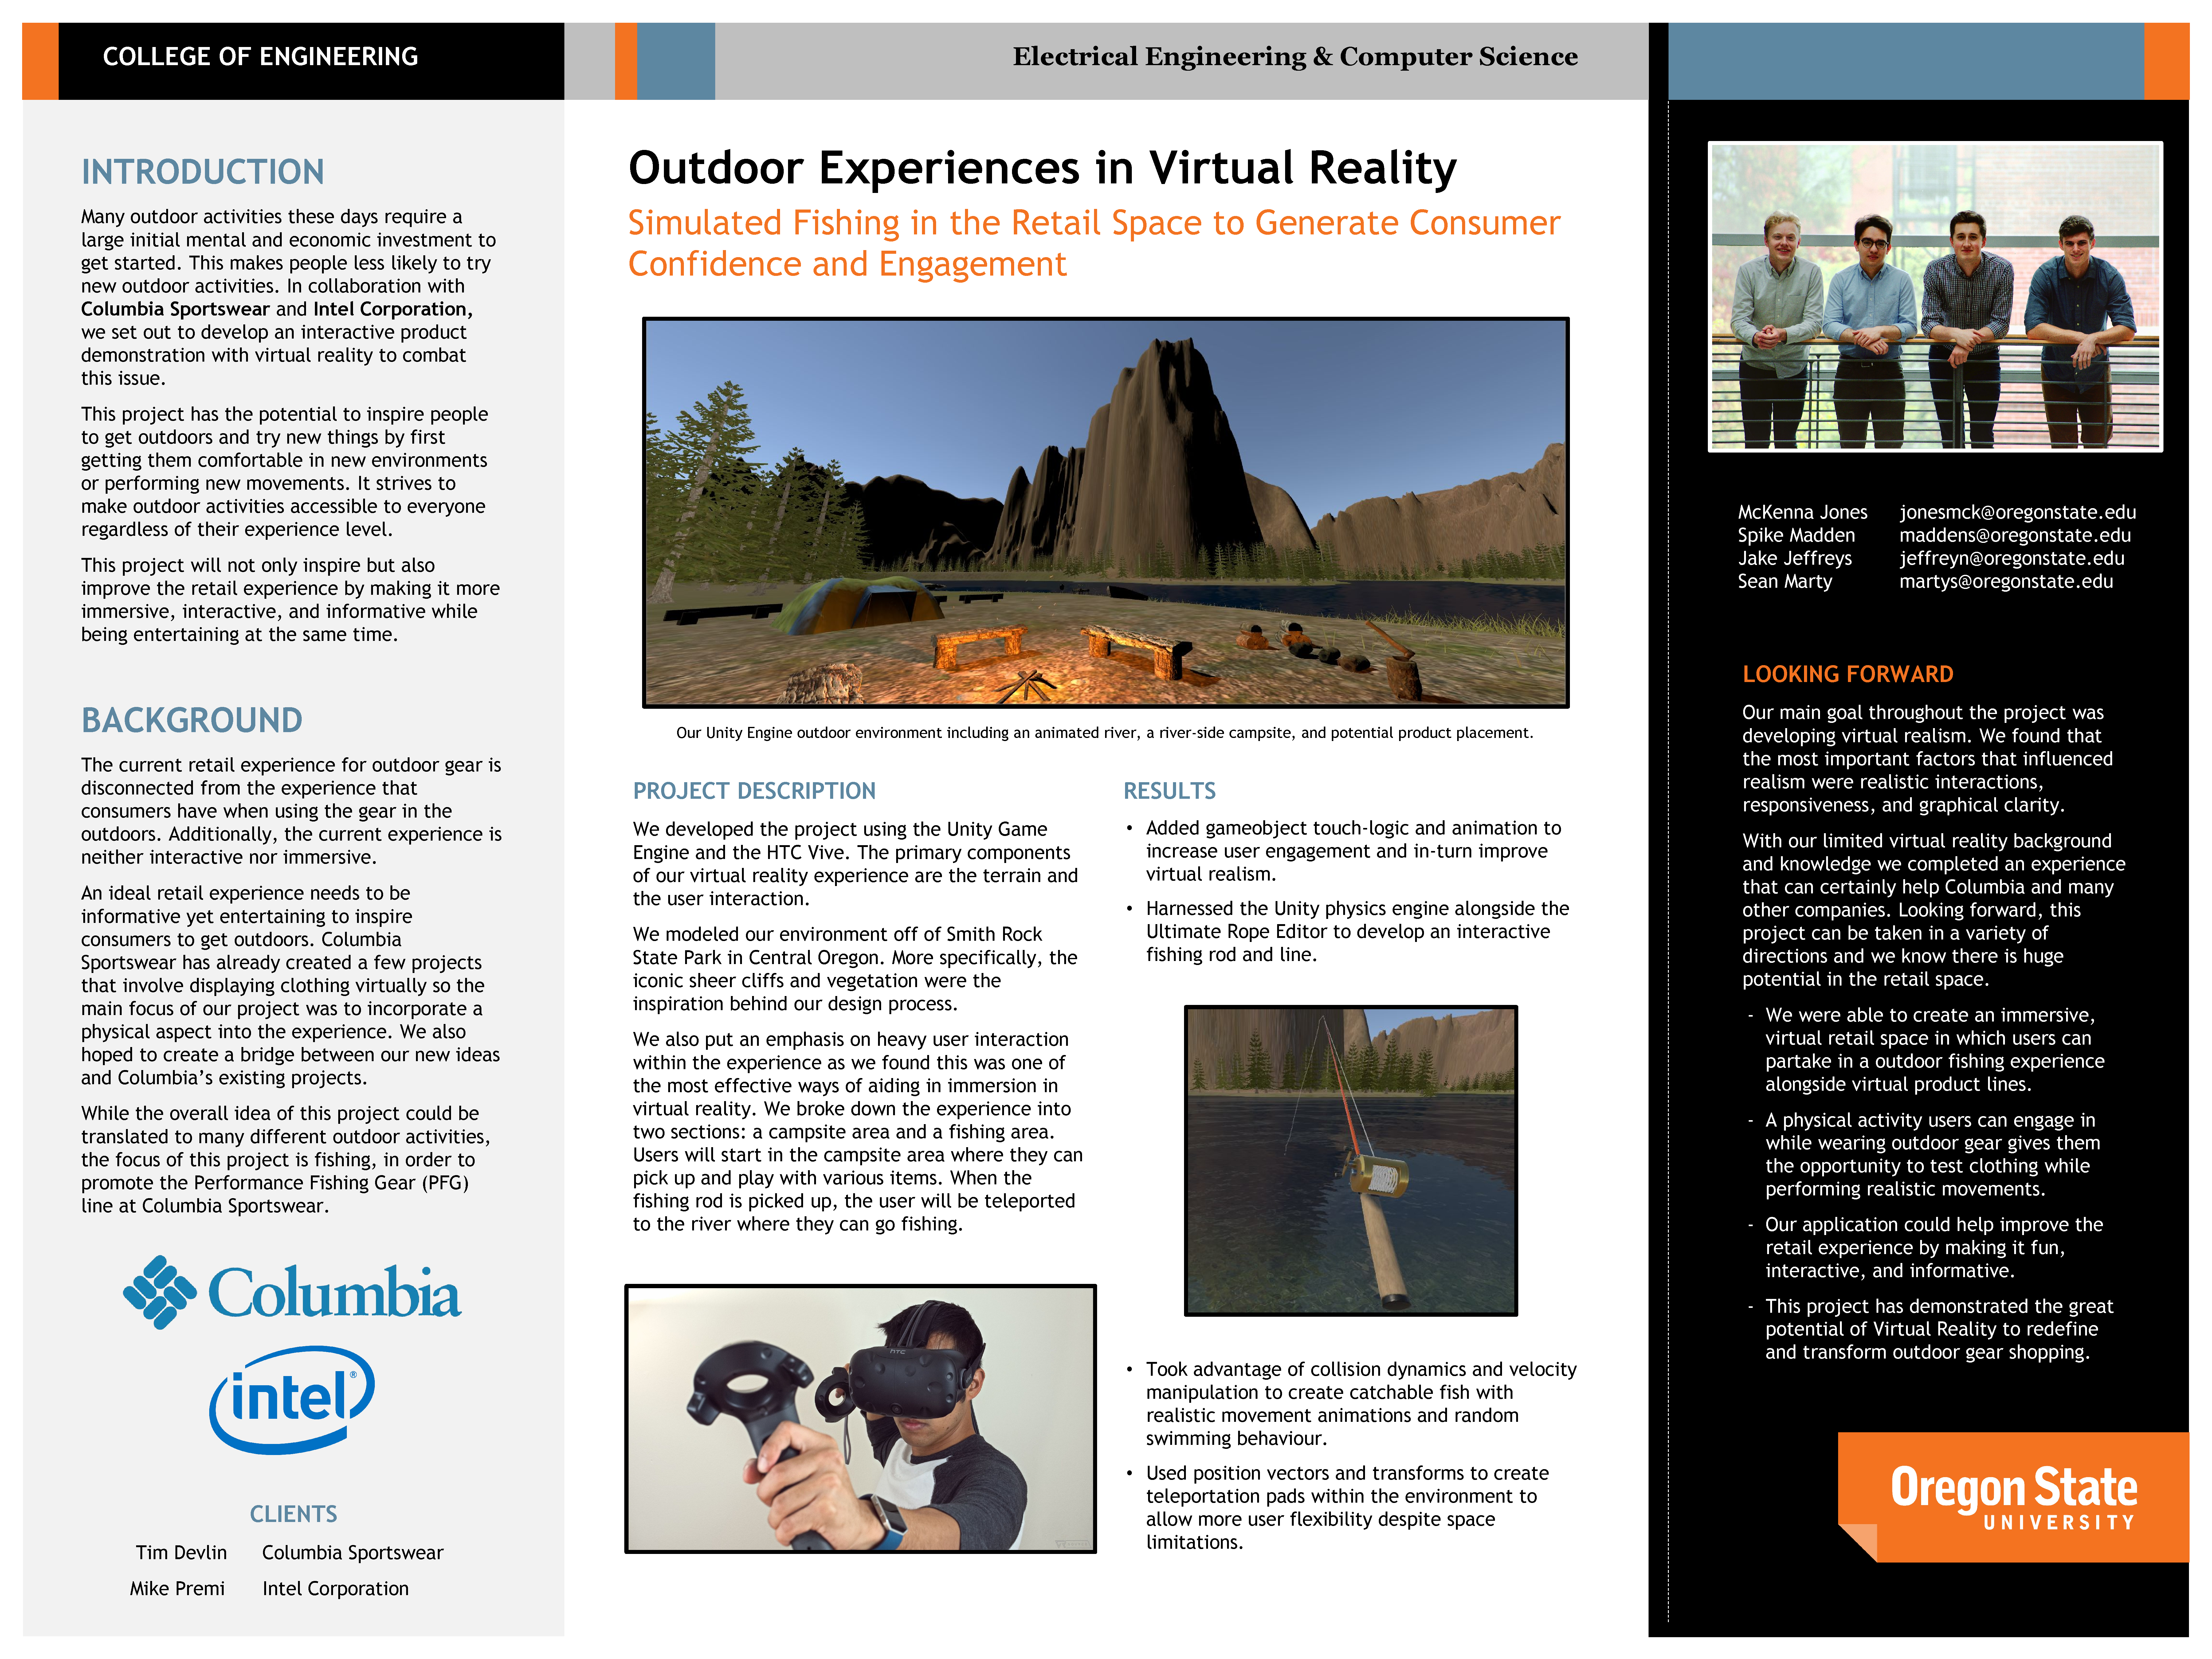
\includepdf[pages=-, frame, scale=1, pagecommand={}, angle=90]{expo_poster.pdf}

% TODO
\section{Project Documentation}
\subsection{Technical Overview}
\subsection{How to Install}
\subsection{Running the Experience}
\subsection{Hardware Requirements}

% TODO
\section{How We Learned}

% TODO (Individually)
\section{What We Learned}
\subsection{Jake}

\subsection{McKenna}
This project was an invaluable learning experience for me. Throughout the process I have learned numerous technical and non technical skills along the way. Overall, I think it was a well rounded project and experience when considering the range of skills I learned. \\

\textbf{Technical Skills}
\begin{itemize}
	\item Unity Game Engine Basics
	\item Virtual Reality development within Unity
	\item SteamVR development within Unity
	\item Unity C\# scripting
	\item Basic physic modeling in Unity
\end{itemize}

\textbf{Non-Technical Skills}
\begin{itemize}
	\item Writing software documentation
	\item Explaining a complex project to a less informed audience (Elevator Pitches)
	\item Team problem solving skills
	\item Project time management
	\item Forming and revising project goals/purposes \\
\end{itemize}

This project has also been a great learning experience regarding project management and working on a team of engineers. If I was to do this project again I would be much more careful when designing the specific requirements of the final product. We definitely overestimated the amount of work that we thought we would be able to complete. This is not inherently bad, as it probably pushed us to complete more than if we had set our expectations low. But the biggest thing that I will now remember is to think realistically when designing a project.

As the project progressed we all learned the importance of working as a more cohesive team. For example, as we began to do more paired programming type work our project began to ramp up much more quickly. As a group I would say that we are all procrastinators at heart. However, as the project went on we did begin to try and finish things a little bit before the final due dates. This definitely reduces stress and results in higher quality work. As far as issues with team members carrying equal weight, the best solution for us was to simply attempt to divide up the work as evenly as possible. This seemed to work with little to no issues.

\subsection{Sean}

\subsection{Spike}

\clearpage
\section{Appendix}
\subsection{Essential Code Listings}
\subsubsection{FishingLineLogic.cs}
This C\# script handles the fishing line, including the reeling in and out motion. It makes use of the UltimateRopeEditor package from the Unity asset store. \\

\begin{minted}[breaklines]{csharp}
using UnityEngine;
using System;
using NewtonVR;

namespace fishingLineLogic
{
    public class FishingLineLogic : MonoBehaviour
    {
        public UltimateRope Rope;
        public Rigidbody FishingRod;
        public float castingSpeed;

        static float m_fRopeExtension;

        void Start()
        {
            m_fRopeExtension = Rope != null ? Rope.m_fCurrentExtension : 0.0f;
        }

        // Called every frame
        void Update()
        {
            bool casting = false;
            bool reelHand = false; // True is right, false is left

            int mag = (int)Math.Round(FishingRod.velocity.magnitude);
            if (mag > 1)
            {
                castingSpeed = mag * 2;
            }
            else
            {
                if (castingSpeed > 0)
                {
                    castingSpeed -= 0.1f;
                }
            }

            if (castingSpeed > 0)
            {
                Debug.Log(castingSpeed);
            }

            // The reel hand is set to the opposite hand of the one that is holding the fishing rod.
            // The user is casting, when the touchpad of the hand that is holding the rod is being pressed.
            if (NVRPlayer.Instance.LeftHand.IsInteracting)
            {
                casting = NVRPlayer.Instance.LeftHand.Inputs[NVRButtons.Touchpad].IsPressed;
                reelHand = true;
            }
            else if (NVRPlayer.Instance.RightHand.IsInteracting)
            {
                casting = NVRPlayer.Instance.RightHand.Inputs[NVRButtons.Touchpad].IsPressed;
                reelHand = false;
            }

            // If the user is casting, set the extension speed
            if (casting)
            {
                m_fRopeExtension += Time.deltaTime * castingSpeed;
            }

            // Find the reel in speed by getting the position of the users thumb on the touchpad.
            if (NVRPlayer.Instance.LeftHand.Inputs[NVRButtons.Touchpad].IsTouched && reelHand == false)
            {
                Vector2 leftAxis = NVRPlayer.Instance.LeftHand.Inputs[NVRButtons.Touchpad].Axis;
                reelIn(leftAxis);
            }
            else if (NVRPlayer.Instance.RightHand.Inputs[NVRButtons.Touchpad].IsTouched && reelHand == true)
            {
                Vector2 rightAxis = NVRPlayer.Instance.RightHand.Inputs[NVRButtons.Touchpad].Axis;

                reelIn(rightAxis);
            }

            // Extend the rope
            if (Rope != null)
            {
                m_fRopeExtension = Mathf.Clamp(m_fRopeExtension, 0.0f, Rope.ExtensibleLength);
                Rope.ExtendRope(UltimateRope.ERopeExtensionMode.LinearExtensionIncrement, m_fRopeExtension - Rope.m_fCurrentExtension);
            }
        }

        // This function sets the speed to reel in the rope, based on the user's position on the touchpad.
        public static void reelIn(Vector2 axis)
        {
            float reelingSpeed;
            if (axis.y > -1 & axis.y < -0.33)
            {
                reelingSpeed = 0.25f;
            }
            else if (axis.y > -0.33 && axis.y < 0.33)
            {
                reelingSpeed = 0.5f;
            }
            else
            {
                reelingSpeed = 0.75f;
            }
            m_fRopeExtension -= Time.deltaTime * reelingSpeed;
        }
    }
}
\end{minted}

\subsubsection{FishLogic.cs}
This script handles the motion of the fish(es), including the catching interaction of the fish.\\

\begin{minted}[breaklines]{csharp}
using NewtonVR;
using System.Collections;
using System.Collections.Generic;
using UnityEngine;

public class FishLogic : MonoBehaviour
{

    public GameObject hook;
    public GameObject lineEnd;
    public bool caught = false;
    public bool userIsFishing = false;
    public GameObject FishParent;
    public bool fishDead = false;

    Vector3 initialPosition;
    FishLogic[] fishList;
    bool otherFishCaught;
    // Use this for initialization
    void Start()
    {
        fishList = FishParent.GetComponentsInChildren<FishLogic>();
        initialPosition = transform.position;
    }

    // Update is called once per frame
    void Update()
    {
        // Check if another fish is currently on the hook
        otherFishCaught = false;
        foreach (FishLogic fish in fishList)
        {
            if (fish.caught == true)
            {
                otherFishCaught = true;
            }
        }

        // Check if fish has not been caught, the user is fishing (hook in water),
        // another fish in not currently on the hook, and the fish isn't dead
        if (!caught && userIsFishing && !fishDead && !otherFishCaught)
        {
            // If hook is 50 units from fish, fish will begin to follow
            if (Vector3.Distance(hook.transform.position, this.transform.position) < 50)
            {
                Vector3 direction = hook.transform.position - this.transform.position;

                direction.y = 0;
                this.transform.rotation = Quaternion.Slerp(this.transform.rotation, Quaternion.LookRotation(direction), .2f * Time.deltaTime);

                if (direction.magnitude > 5)
                {
                    this.transform.Translate(0, 0, 0.1f);
                }

                // When hook is close enough, lock onto hook, with a character joint
                // if another fish is not currently not on the hook.
                else if (direction.magnitude <= 5 && !otherFishCaught)
                {
                    caught = true;
                    this.gameObject.AddComponent<CharacterJoint>();
                    CharacterJoint joint = this.GetComponent<CharacterJoint>();
                    joint.autoConfigureConnectedAnchor = false;
                    joint.connectedAnchor = new Vector3(0, 0, 3f);

                    Rigidbody lineEndRigid = lineEnd.GetComponent<Rigidbody>();

                    this.transform.position = lineEnd.transform.position;
                    joint.connectedBody = hook.GetComponent<Rigidbody>();

                    Rigidbody fishRigid = this.GetComponent<Rigidbody>();
                    fishRigid.isKinematic = false;

                    // Move every other fish back to their initial position
                    foreach (FishLogic fish in fishList)
                    {
                        if (fish.gameObject.name != this.name && !fish.fishDead)
                        {
                            fish.gameObject.transform.position = fish.initialPosition;
                        }
                    }
                }
            }

            // If there is a character joint on the fish, it is currently attatched to the hook.
            // Vibrate the controller, while it is.
            if (this.GetComponent<CharacterJoint>())
            {
                if (NVRPlayer.Instance.LeftHand.IsInteracting)
                {
                    NVRPlayer.Instance.LeftHand.TriggerHapticPulse(1500, NVRButtons.Touchpad);
                }
                else if (NVRPlayer.Instance.RightHand.IsInteracting)
                {
                    NVRPlayer.Instance.RightHand.TriggerHapticPulse(1500, NVRButtons.Touchpad);
                }
                return;
            }
        }
    }
}
\end{minted}

\subsection{Images}
Below are some images that show the current state of our virtual reality experience.

\vspace{1cm}

\begin{figure}[h]
    \centering
    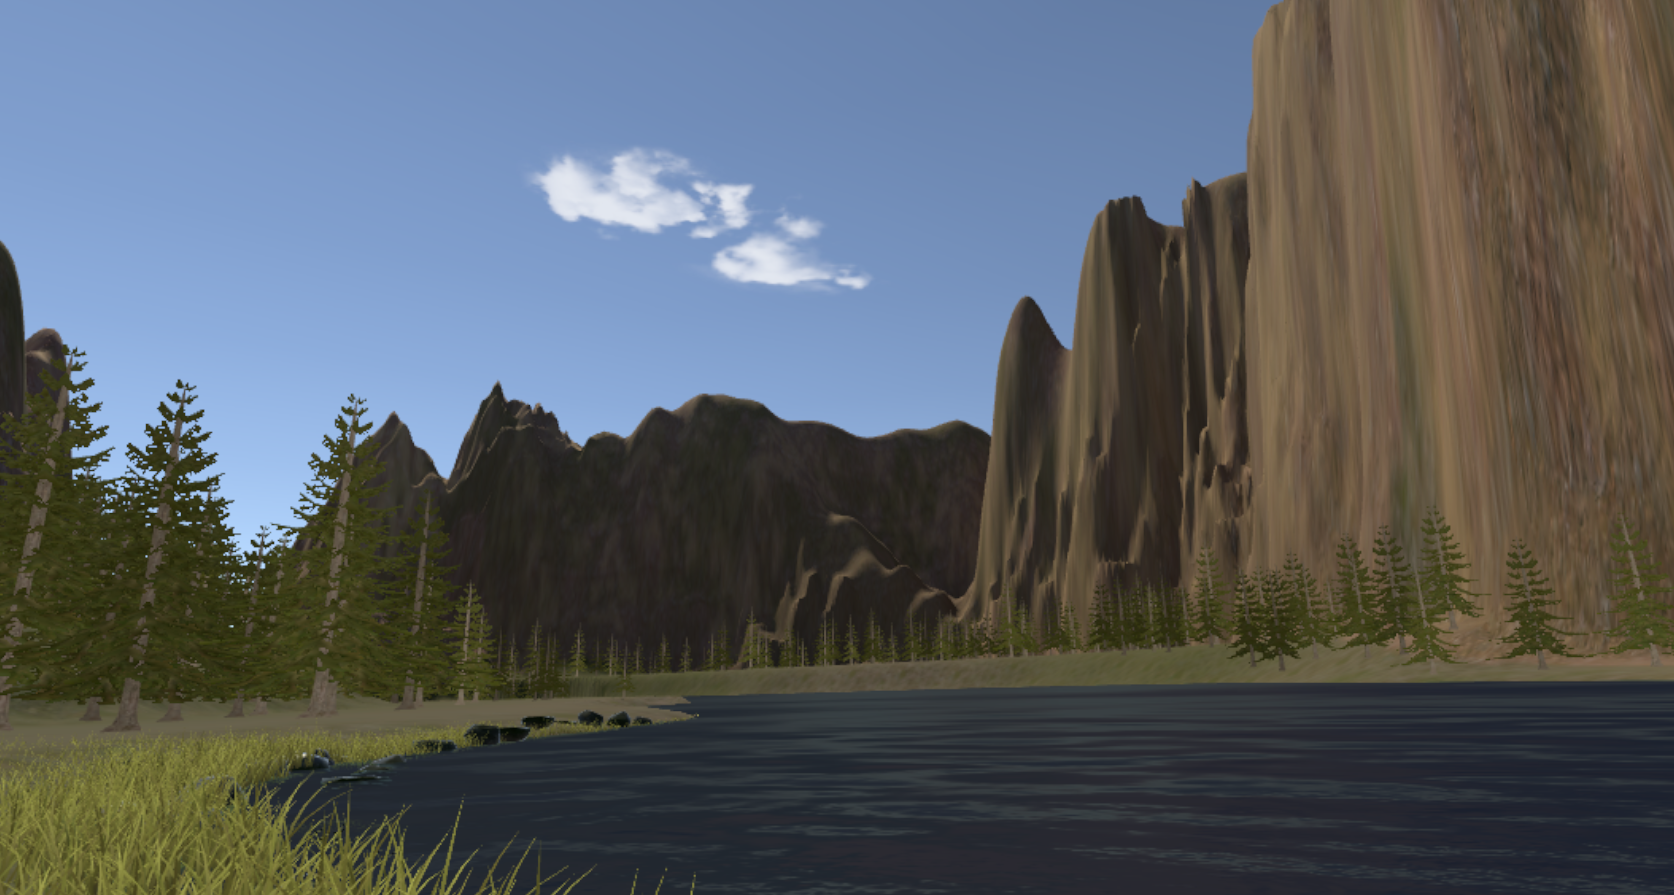
\includegraphics[width=0.80\textwidth]{waterLeft.png}
    \caption{Image of our landscape}
\end{figure}

\begin{figure}[h]
    \centering
    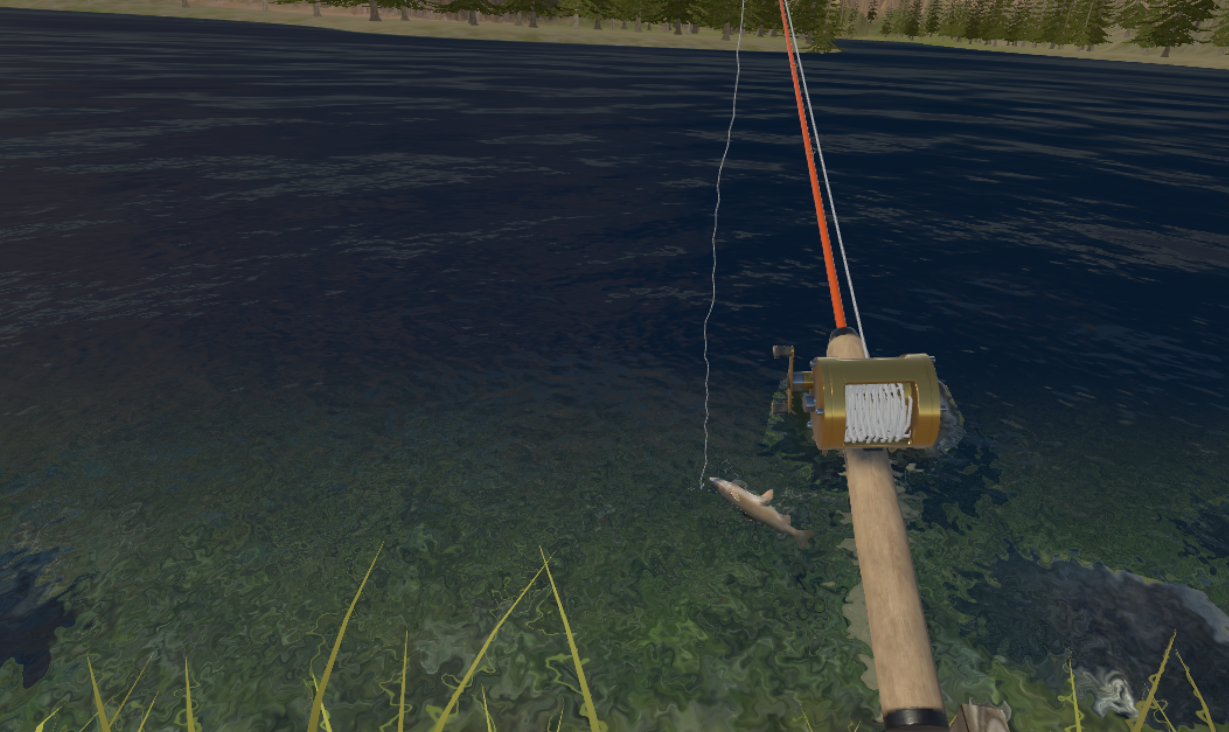
\includegraphics[width=0.8\textwidth]{fishOnLine.png}
    \caption{Fishing rod and line with fish on it}
\end{figure}

\begin{figure}[h]
    \centering
    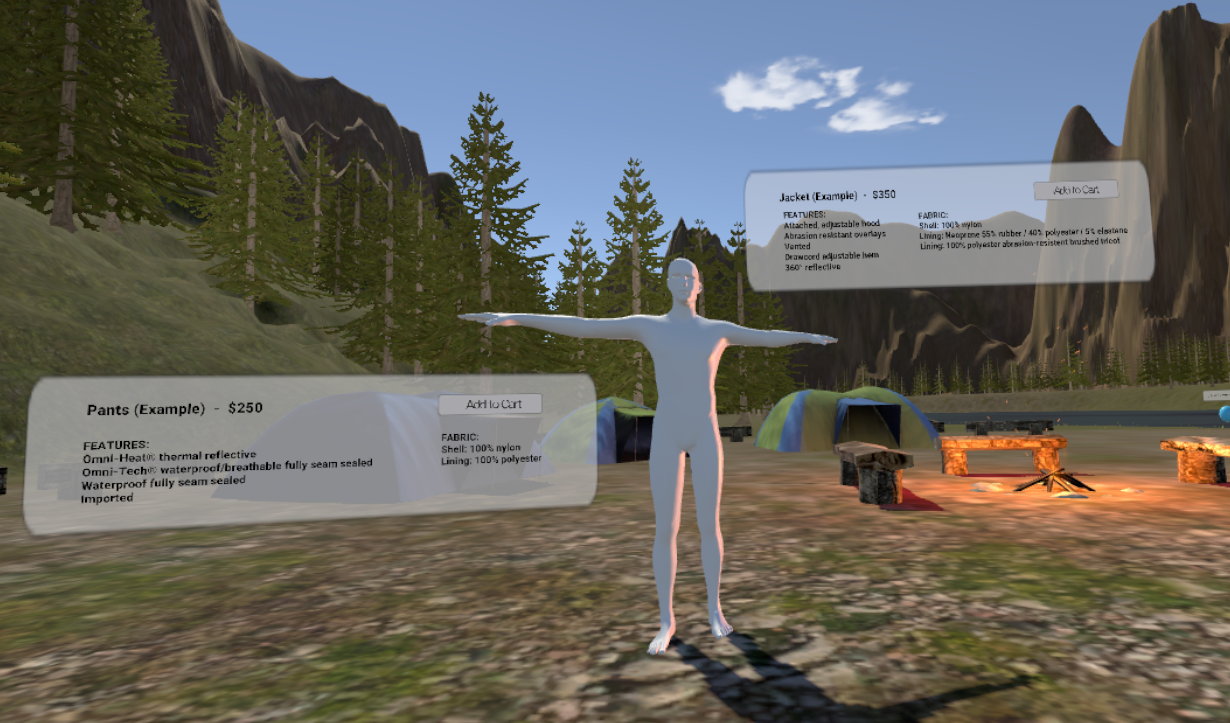
\includegraphics[width=0.8\textwidth]{gearPrototype.png}
    \caption{Campsite with placeholder gear information}
\end{figure}

% \bibliographystyle{IEEEtran}
% \bibliography{}
\end{document}
